\documentclass[12pt,a4paper]{report}

\usepackage{styles/dolgozat}

\usepackage{listings}
\usepackage{styles/cpp}
\usepackage{styles/javascript}
\usepackage{styles/python}
\usepackage{styles/sql}
\usepackage{styles/json}

\usepackage{hyperref}
\usepackage{url}

\begin{document}

\pagestyle{empty} %a címlapon ne legyen semmi=empty, azaz nincs fejléc és lábléc

% A Miskolci Egyetem címere
{\large
\begin{center}
\vglue 1truecm
\textbf{\huge\textsc{Szakdolgozat}}\\
\vglue 1truecm

\includegraphics[width=4.8truecm, height=4truecm]{images/me_logo.png}\\
\textbf{\textsc{Miskolci Egyetem}}
\end{center}}

\vglue 1.5truecm %függõleges helykihagyás

% A szakdolgozat címe, akár több sorban is
{\LARGE
\begin{center}
\textbf{A szakdolgozat címe}
\end{center}}

\vspace*{2.5truecm}
% A hallgató neve, évfolyam, szak(ok), a konzulens(ek) neve
{\large
\begin{center}
\begin{tabular}{c}
\textbf{Készítette:}\\
Szakdolgozó Neve\\
Programtervező informatikus
\end{tabular}
\end{center}
\begin{center}
\begin{tabular}{c}
\textbf{Témavezető:}\\
Piller Imre
\end{tabular}
\end{center}}
\vfill
% Keltezés: Hely, év
{\large
\begin{center}
\textbf{\textsc{Miskolc, 2020}}
\end{center}}

\newpage


\newpage

\pagestyle{empty}

%Feladatkiiras
\begin{flushleft}
\textsc{\bfseries Miskolci Egyetem}\\
Gépészmérnöki és Informatikai Kar\\
Alkalmazott Matematikai Intézeti Tanszék\hspace*{4cm}\hfil \textbf{Szám:}
\end{flushleft}
\vskip 0.5cm
\begin{center}
\large\textsc{\bfseries Szakdolgozat Feladat}
\end{center}
\vskip 0.5cm
Utry Máté Attila (YR10UU) programtervező informatikus jelölt részére.\newline

\noindent\textbf{A szakdolgozat tárgyköre:} kulcsszavak, hasonlók\newline

\noindent\textbf{A szakdolgozat címe:} Webalkalmazás fejlesztése szervezeti folyamatok kezeléséhez\newline

\noindent\textbf{A feladat részletezése:}

\medskip

\emph{A különféle szervezetek (például intézmények, vállalatok) ügymenete nagyon bonyolult, és egyedi. A dolgozat egy olyan alkalmazás elkészítésének bemutatását célozza, amely konkrét szervezeti formától függetlenül képes azok folyamatainak modellezéséhez eszközt biztosítani.}

\medskip

\emph{A folyamatok alatt itt elsősorban olyan, véges állapotú automatával leírható műveletsorokat értünk, amely esetenként további, összetettebb (például szerepkörökhöz) kötött feltételek, külső állapotok teljesülését is szükségessé teszik. A dolgozatban ezen állapotgép és feltételrendszer leírási módjához szükséges alkalmazást kell megtervezni és implementálni.}

\medskip

\emph{Az alkalmazásnak webes környezetben, szerver-kliens architektúrának megfelelően kell elkészülnie. Ehhez szerver oldalon a Falcon nevű, Python alapú mikrokeretrendszer ad alapot, míg a kliens megvalósításához egy elterjedt JavaScript alapú keretrendszert kell használni. Az adatokat az alkalmazásnak relációs adatbázisban kell tárolnia.}

\vfill

\noindent\textbf{Témavezető:} Piller Imre (egyetemi tanársegéd) \newline

% \noindent\textbf{Konzulens(ek):} (akkor kötelezõ, ha a témavezetõ nem valamelyik matematikai tanszékrõl való; de persze lehet egyébként is)\newline

\noindent\textbf{A feladat kiadásának ideje:}\newline

%\noindent\textbf{A feladat beadásának határideje:}

\vskip 2cm

\hbox to \hsize{\hfil{\hbox to 6cm {\dotfill}\hbox to 1cm{}}}

\hbox to \hsize{\hfil\hbox to 3cm {szakfelelős}\hbox to 2cm{}}

\newpage

\vspace*{1cm}  
\begin{center}
\large\textsc{\bfseries Eredetiségi Nyilatkozat}
\end{center}
\vspace*{2cm}  

Alulírott \textbf{Utry Máté Attila}; Neptun-kód: \texttt{YR10UU} a Miskolci Egyetem Gépészmérnöki és Informatikai Karának végzős Programtervező informatikus szakos hallgatója ezennel büntetőjogi és fegyelmi felelősségem tudatában nyilatkozom és aláírásommal igazolom, hogy \textit{Webalkalmazás fejlesztése szervezeti folyamatok kezeléséhez}
című szakdolgozatom saját, önálló munkám; az abban hivatkozott szakirodalom
felhasználása a forráskezelés szabályai szerint történt.\\

Tudomásul veszem, hogy szakdolgozat esetén plágiumnak számít:
\begin{itemize}
\item szószerinti idézet közlése idézőjel és hivatkozás megjelölése nélkül;
\item tartalmi idézet hivatkozás megjelölése nélkül;
\item más publikált gondolatainak saját gondolatként való feltüntetése.
\end{itemize}

Alulírott kijelentem, hogy a plágium fogalmát megismertem, és tudomásul veszem, hogy
plágium esetén szakdolgozatom visszautasításra kerül.

\vspace*{3cm}

\noindent Miskolc, \hbox to 2cm{\dotfill} .év \hbox to 2cm{\dotfill} .hó \hbox to 2cm{\dotfill} .nap

\vspace*{3cm}

\hspace*{8cm}\begin{tabular}{c}
\hbox to 6cm{\dotfill}\\
Hallgató
\end{tabular}



\newpage

\noindent 1.

\begin{tabular}{cl}
&szükséges (módosítás külön lapon) \\
A szakdolgozat feladat módosítása& \\
& nem szükséges\\
&\\
\hbox to 4cm{\dotfill}&\multicolumn{1}{c}{\hbox to 5cm{\dotfill}}\\
dátum& \multicolumn{1}{c}{témavezető(k)}
\end{tabular}
\vskip1.5mm

\noindent 2. A feladat kidolgozását ellenőriztem:

\vskip1.5mm

\begin{tabular}{l@{\hspace*{4cm}}l}
témavezető (dátum, aláírás):& konzulens (dátum, aláírás):\\
\dotfill&\dotfill\\
\dotfill&\dotfill\\
\dotfill&\dotfill
\end{tabular}

\vskip1.5mm

\noindent 3. A szakdolgozat beadható:

\vskip1.5mm

\begin{tabular}{@{\hspace*{1.3cm}}c@{\hspace*{2.1cm}}c}
\hbox to 4cm{\dotfill}&\multicolumn{1}{c}{\hbox to 5cm{\dotfill}}\\
dátum& \multicolumn{1}{c}{témavezető(k)}
\end{tabular}

\vskip1.5mm

\noindent 4.
\begin{tabular}[t]{@{}l@{\hspace*{1mm}}l@{\hspace*{1mm}}l@{}}
A szakdolgozat& \hbox to 3.5cm{\dotfill} &szövegoldalt\\
              & \hbox to 3.5cm{\dotfill} &program protokollt (listát, felhasználói leírást)\\
              &\hbox to 3.5cm{\dotfill}   &elektronikus adathordozót (részletezve)\\
              &\hbox to 3.5cm{\dotfill} & \\
              &\hbox to 3.5cm{\dotfill} &egyéb mellékletet (részletezve)\\
              &\hbox to 3.5cm{\dotfill} &\\
\end{tabular}
\newline tartalmaz.

\vskip1.5mm

\begin{tabular}{@{\hspace*{1.3cm}}c@{\hspace*{2.1cm}}c}
\hbox to 4cm{\dotfill}&\multicolumn{1}{c}{\hbox to 5cm{\dotfill}}\\
dátum& \multicolumn{1}{c}{témavezető(k)}
\end{tabular}

\noindent 5.

\begin{tabular}{ll}
&bocsátható\\
A szakdolgozat bírálatra& \\
& nem bocsátható\\
\end{tabular}

\vskip1.5mm

\noindent A bíráló neve: \hbox to 8cm{\dotfill}

\vskip4mm

\begin{tabular}{@{\hspace*{1.3cm}}c@{\hspace*{2.1cm}}c}
\hbox to 4cm{\dotfill}&\multicolumn{1}{c}{\hbox to 5cm{\dotfill}}\\
dátum& \multicolumn{1}{c}{szakfelelős}
\end{tabular}

\noindent 6.
\begin{tabular}[t]{@{}l@{\hspace*{1mm}}l@{\hspace*{1mm}}l@{}}
A szakdolgozat osztályzata& &\\
&a témavezető javaslata:& \hbox to 3cm{\dotfill}\\
&a bíráló javaslata:& \hbox to 3cm{\dotfill}\\
&a szakdolgozat végleges eredménye:& \hbox to 3cm{\dotfill}
\end{tabular}

\vspace*{4mm}

\noindent Miskolc, \hbox to 4.5cm{\dotfill} \hspace*{2.5cm}
\begin{tabular}[t]{cc}
\hbox to 6cm{\dotfill}\\
a Záróvizsga Bizottság Elnöke
\end{tabular}


\cleardoublepage
\pagenumbering{gobble}
\tableofcontents
\cleardoublepage
\pagenumbering{arabic}

\newpage

\pagestyle{fancy}

\Chapter{Bevezetés}

A szakdolgozat egy szervezeti folyamatok modellezését elősegítő gráf szerkesztő alkalmazást mutat be. Egy szervezet életében nagyon sok folyamattal lehet találkozni napi szinten, melyek sokasága és hatékony végrehajtása érdekében célszerű lehet azokat valamilyen folyamatkezelő program segítségével ábrázolni.

Több folyamatmodellezésre használható, készen elérhető alkalmazás létezik már. Akkor miért volt szükség még egy elkészítésére a szakdolgozat keretein belül? Többek között erre a kérdésre is választ fogunk kapni a szakdolgozat elolvasása után.

Az első tartalmi fejezet általános áttekintést ad az üzleti (szervezeti) folyamatokról, illetve azok modellezéséről. Az ezt követő fejezetek az alkalmazás tervezési folyamatait, megvalósítását, valamint használatát írja le. Végül ez utóbbi könnyebb megértése érdekében néhány gyakorlati példa segítségével szemlélteti, hogy hogyan történik a folyamatmodellezés az alkalmazás segítségével.
\Chapter{Üzleti folyamatok és modellezésük}

%általános áttekintést kellene adjon arról, hogy mik azok az üzleti folyamatok, hogyan szokták modellezni őket, milyen matematikai modellek vannak, egyáltalán miért lényeges, milyen szoftveres eszközök vannak.

Dolgozatom első tartalmi fejezetének alapjául a(z) \cite{xflower} forrás blogbejegyzéseit használtam, ezeket dolgoztam fel és egészítettem ki önálló gondolatokkal.

\Section{Mik azok az üzleti folyamatok?}

Elsőként nézzük meg, mit nevezhetünk egy folyamatnak. A folyamat szó más-más jelentéssel bír annak függvényében, hogy hol használjuk: például mást jelent a hétköznapi életben, mint az informatikában. A mi esetünkben a folyamat előre meghatározott vagy tetszőleges sorrendben elvégezhető tevékenységek kapcsolatrendszerét jelenti.

Tehát gyakorlatilag a folyamat olyan tevékenységek halmaza, amelyek egymással kölcsönhatásba lépnek egy adott cél elérése érdekében. Ezt a jelentését használhatjuk az üzleti folyamatokra is, hiszen ha egy üzleti célt tűzünk ki magunk elé, akkor annak megvalósulása is több tevékenység egymásutániságából, több lépésből fog adódni. Ezeket a lépéseket együttesen nevezzük \textit{üzleti folyamat}nak.

Alapvetően kétféle megközelítése van a lépések végrehajtása sorrendjének:

\begin{itemize}
\item Tevékenységek tetszőleges sorrendben elvégezhetőek.
\item Csak egymás utáni, meghatározott sorrendben követhetik egymást.
\end{itemize}

Az üzleti folyamatok minden vállalat életében napi szinten jelen vannak és egy áttekinthető láncolatot alkotnak a termék előállításához szükséges nyersanyagok beszerzésétől kezdve a munkafolyamatokon keresztül egészen a piacra kerülésig, és a piacon való sikeres vagy sikertelen szereplésig.

Üzleti folyamatokról általában akkor beszélünk, ha egy adott vállalat termékét, szolgáltatását, vagy menedzsmentjét akarjuk elhelyezni a gazdasági életben. Belátható, hogy a termék minősége és mennyisége összefügg a gyártó menedzsmentjének arculatával, piaci ismertségével, és a termék iránti kereslet erejével. Ezeket az összefüggéseket jeleníti meg egy vállalat reklám, PR, és marketing tevékenysége. Közismert példa, hogy az MGM stúdió világviszonylatban piacvezető termékeket (filmeket) állít elő, de reklámköltsége meghaladja a filmgyártás és forgalmazás költségeit.

Hogy érthetőbb legyen mit is jelent a gyakorlatban az üzleti folyamat, nézzünk rá egy egyszerű példát:

Adott egy startup (vagy magyarosabban \textit{korai fázisú vállalkozás}\cite{wiki}), ahol szükségessé válik bizonyos irodaszerek beszerzése. Magát a beszerzés menetét egy kizárólag kötött sorrendben elvégezhető folyamat fogja leírni. Nézzük a folyamat lépéseit:

\begin{enumerate}
\item Első lépésben konkrétan meghatározzuk, hogy melyek azok az eszközök, amelyekre szükség van, és miből hány darab szükségeltetik. Ezeknek az összeírása az első feladat.

\item Miután összegyűjtöttük a megrendelendő tárgyakat, meg kell vizsgálnunk, hogy a vállalkozás mekkora anyagi kerettel rendelkezik, és ebből mennyit tudunk a megrendelésre költeni. Ha rendelkezünk megfelelő pénzösszeggel, akkor minden rendben van, tovább lehet lépni. Ha viszont nem, akkor valamilyen szempont alapján ki kell húzni a listáról bizonyos termékeket (például a legszükségtelenebbeket). Ez utóbbi termékek megrendelése vagy elvetése a következő lépéstől is függ.

\item Ha már rendelkezésünkre áll a lista és a pénzügyi fedezet, utána kell néznünk, hogy az adott eszközök hol szerezhetőek be a legalacsonyabb áron (ehhez segítséget tud nyújtani például az Árukereső\cite{arukereso} weboldala, ami ár szerinti növekvő sorrendben kilistázza, hogy egy adott termék mely online webáruházakban és milyen áron érhetők el). Természetesen nem csak az alacsony ár, hanem más szempont is szóba jöhet (például a garancia időtartama az adott termékre, a kiszállítás díja, stb.).

Ennél a lépésnél derül ki, hogy pontosan mennyi összeget kell a meglévő pénzügyi keretből az új eszközök megrendelésére fordítani. Lehetséges, hogy marad még pénz egy korábban az anyagi keret szűkösségére való hivatkozás miatt lehúzott termék megvásárlására.

\item Mindezek után elindulhat a megrendelés folyamata. Ez többféleképpen is történhet:

\begin{itemize}
\item Az eszközöket online rendeljük meg. Ennek előnye, hogy egyszerre több helyen is megfigyelhetjük a termékeket, utána járhatunk az azokat árusító weboldalak hitelességének, megbízhatóságának, véleményeket olvashatunk róla, és nem kell személyesen megjelennünk az adott áruházban. Hátránya, hogy időbe telik a termékek kiszállítása, és adott esetben számolnunk kell a szállítási költséggel is. Ez utóbbinak mértéke áruházanként eltérő. Ugyanakkor ma már léteznek olyan webáruházak is, ahol a megrendelt terméket személyesen is át lehet venni egy előre meghatározott üzlethelységben, így azokhoz gyorsabban juthatunk hozzá, viszont ebben az esetben a megrendelőre hárul a szállítási költség.

\item Megtehetjük, hogy nem rendeljük meg előzetesen a termékeket, hanem azok beszerzésére személyesen megyünk be az áruházakba. Ezt akkor célszerű alkalmaznunk, mikor egy nagyobb áruházat fogunk meglátogatni, ahol nagy eséllyel az összes termék rendelkezésünkre fog állni, így azokat egy helyről azonnal meg is tudjuk venni, és elvinni. Nagy előny ebben az esetben (szemben az online rendeléssel), hogy ki is tudjuk próbálni az adott termékeket, hogy hogyan működnek, van-e valamilyen hibájuk.
\end{itemize}

\item Ezek után, hogy a megrendelt termékek eljutottak az irodába, utolsó lépésként már csak szét kell osztani azokat aszerint, hogy mely terméket ki igényelte.
\end{enumerate}
Ezzel a végére is értünk egy egyszerűbb üzleti folyamatnak.

Azért ezt a fenti példát hoztam szemléltetésként, mert ez valamilyen formában minden vállalkozásnál jelen van. Ha jobban belegondolunk, láthatjuk, hogy gyakorlatilag szinte minden tevékenységet (így adott termék vagy termékek beszerzését is) folyamatban végzünk. Fontos megjegyezni, hogy ennél a példánál, és az ehhez hasonlóknál a lépéseket csak adott sorrendben hajthatjuk végre. Például nem vihetünk el egy terméket az áruházból úgy, hogy csak majd később fizetünk érte.

\begin{figure}[h]
\centering

\includegraphics[scale=0.5]{images/uzleti_intelligencia.png}
\caption{Üzleti intelligencia\cite{piacp}}
\label{fig:uzlint}
\end{figure}

\Section{Üzleti folyamatok modellezése}

Az előző részben olvashattuk, hogy nagyon sok mindent folyamatban végzünk. Akár egy legegyszerűbb hétköznapi tevékenységet is. Egy vállalat esetében pedig az ilyen tevékenységekből jóval több van, melyek lényeges szerepet játszanak annak működésében. Emiatt fontos az, hogy a vállalat bizonyos folyamatai rögzítésre kerüljenek. Ezért van szükség a folyamatok \textit{modellezésére}. Ennek egy egyszerű, átlátható formája a folyamatábra használata.

\SubSection{Modellezés folyamatábrával}

A folyamatábra gyakorlatilag egy olyan eszköz, amely segítségével grafikusan ábrázolhatóak a tevékenységek, folyamatok. A különböző folyamatokat különböző szimbólumokkal jelölhetjük rajta, közöttük sorrendiséget állíthatunk fel meghatározva ezáltal azt, hogy időben melyik esemény melyik után vagy előtt következik be. Hogy érthetőbb legyen, miről is van szó, \aref{fig:folyamata} ábra egy nagyon egyszerű folyamatábrát szemléltet, amin a szakdolgozatom készítésének legfőbb lépései helyezkednek el.

\begin{figure}[h]
\centering
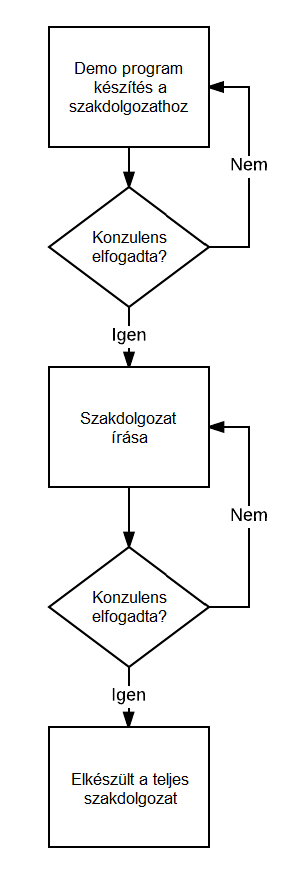
\includegraphics[scale=0.7]{images/folyamatabra.png}
\caption{Egy egyszerű folyamatábra}
\label{fig:folyamata}
\end{figure}

\newpage

A fent látható folyamatábra egyszerűségét az is adja, hogy nem teljes. Nincsen kiindulópontja, sem végpontja. Olyan, mintha egy nagyobb folyamatból csak néhány tevékenységet ábrázolnánk. Ahhoz, hogy teljes legyen a folyamatábra, szükség van kezdő- és végállapotra.

Nézzük tehát, hogy mitől lesz teljes egy folyamatábra, illetve hogy általánosságban milyen részeket tartalmaz. Az alábbi (leggyakoribb, szinte minden folyamatábrán megtalálható) szimbólumok a következő jelentéssel bírnak:

\begin{itemize}
\item \textit{Téglalap} jelöli a tevékenységet. Ebből van a legtöbb a folyamatábrán, hiszen ezek szemléltetik magát a folyamatot, az események egymás utáni történését.
\item \textit{Rombusz} alak jelenti az átjárókat. Ezek útválasztóként funkcionálnak azáltal, hogy egy feltételt szabnak meg, melynek kiértékelésétől függ, hogy melyik tevékenység fog következni. Általában két másik tevékenység követi, amelyek közül az lesz a soron következő, amelyikre az útválasztó kiértékelése a megfelelő (igaz vagy hamis) értéket adja.
\item \textit{Üres fehér kör vékony fekete körívvel} fejezi ki a "START" állapotot \textit{(kezdőállapot)}. Itt kezdődik el a reprezentált folyamat. Legalább egy "START" szimbólumot tartalmaznia kell minden teljes folyamatábrának.
\item A folyamat befejezését az \textit{üres fehér kör vastag fekete körívvel} jelöli. Ezt "END" állapotnak \textit{(végállapotnak)} is szokták nevezni. Ebből is legalább egynek lennie kell ahhoz, hogy teljes legyen a folyamatábra, hiszen ahogy elkezdődik egy folyamat, úgy az be is fejeződik egy bizonyos idő után. Előfordul olyan folyamatábra, ami több végállapotot tartalmaz, mint kezdőállapotot. Ez nem hiba, hiszen a való életben is gyakran fejeződik be egy elkezdett folyamat többféleképpen.
\item A különböző folyamatokat vonalak kötik össze, melyeket \textit{szekvenciafolyam}nak neveznek. Fontos, hogy ezek nem lehetnek csak vonalak nyíl nélkül, hiszen egyértelműen meg kell határozniuk, hogy melyik tevékenységből melyik másik következik.
\end{itemize}

Példaként tekintsük \aref{fig:uresfolyamat} ábrát, ami egy teljes folyamatábrát mutat, mely a fent említett szimbólumok közül mindegyikből tartalmaz legalább egyet (beleértve a kezdő- és végállapotokat is).

\begin{figure}[h]
\centering
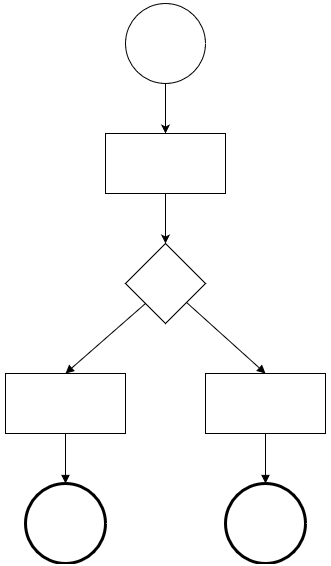
\includegraphics[scale=0.8]{images/uresfolyamat.png}
\caption{Egy üres, de teljes folyamatábra (Forrás: \cite{drawio}}
\label{fig:uresfolyamat}
\end{figure}

Természetesen léteznek ennél sokkal összetettebb, többféle szimbólumot tartalmazó folyamatábrák is, azonban már egy ekkora ábrán is meg lehet jeleníteni egyszerűbb üzleti folyamatokat.

\Section{Egy folyamatokat szemléltető szoftveres eszköz}

\SubSection{Draw.io}

Folyamatok ábrázolására már nagyon sok kész program létezik. Például \aref{fig:uresfolyamat} ábrát is egy ilyen folyamatábrázoló szoftver segítségével készítettem el, melynek neve \textit{Draw.io}\cite{drawio}. A Draw.io a legismertebb és legsokoldalúbb ingyenes folyamatábrázoló alkalmazás. Az alkalmazás nem igényel letöltést, a böngésző segítségével el tudjuk érni akár a rövidebb \url{www.draw.io} URL címen keresztül. További előnye még, hogy regisztrációt sem igényel, hanem azonnal az oldal betöltése után már kezdhetjük is a folyamataink modellezését.

\begin{figure}[h]
\centering
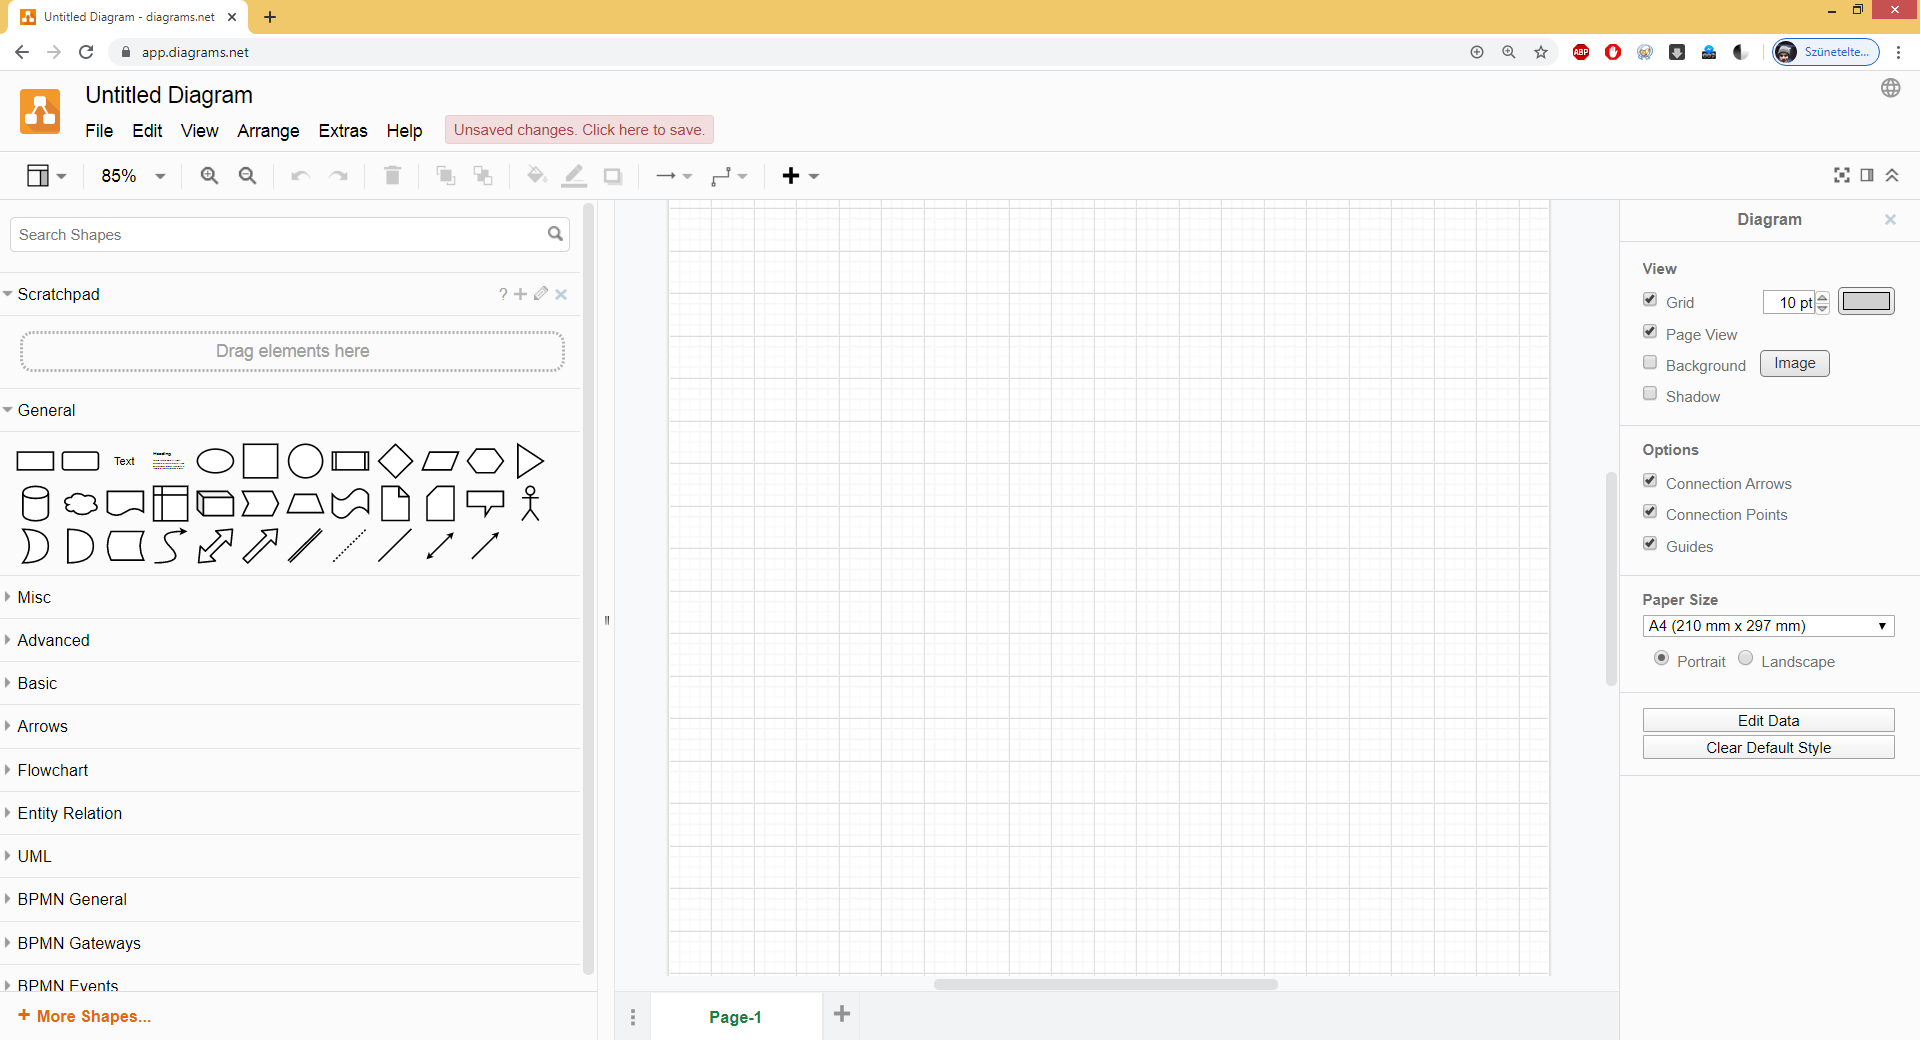
\includegraphics[scale=0.3]{images/drawio.png}
\caption{A Draw.io nyitóoldala (Forrás:\cite{drawio})}
\label{fig:drawio}
\end{figure}

Láthatjuk, hogy rengeteg lehetőség tárul elénk. A modellezéshez nagyon sok féle szimbólum közül választhatunk számunkra megfelelőt. Természetesen mindegyik más jelentéssel bír, azonban a program teljes egészében a felhasználóra bízza azok használatát: nem határoz meg integritási feltételeket, így a felhasználó szabályoktól függetlenül alakíthat ki számára kedvező ábrákat.

Használata viszonylag egyszerű, felhasználóbarát. A felhasználó kiválaszt egy elemet a bal oldali eszköztárból, és azt kattintással, vagy akár behúzással megjeleníti a képernyő közepén található négyzetrácsos részen. Az így megjelenített szimbólumokat nyomva tartott bal egérgomb mellett az egér mozgatásával lehet áthelyezni.

Az általános szimbólumokon kívül (amik a program bal oldali menüjében le vannak nyitva \textit{General} néven) különböző nyilakat, egyéb formákat használhatunk, UML diagramokat készíthetünk, illetve az üzleti folyamatmodell és jelölés (\textit{Business Process Model and Notation}, BPMN) sajátos alakzatait is igénybe vehetjük. De ha még ez se lenne elég, akkor lehetőség van az eszköztárat kibővíteni további alakzatok hozzáadásával, amit a bal alsó sarokban található \textbf{"More Shapes\ldots"} (további alakzatok) gomb megnyomásával érhetünk el.

Elkészített folyamatábráink / diagramjaink mentésére is többféle módot kínál az alkalmazás. Lehetőség van PNG, SVG, HTML, és XML formátumba is menteni a munkánkat, amiket a saját eszközünkre, vagy akár Google Drive-ra, GitHub-ra, és még sokféle felületre azonnal exportálhatunk is.

Összegezve tehát a Draw.io egy rendkívül hasznos és változatos alkalmazás, amely sokféle megvalósítási lehetőséget kínál a felhasználók számára. Egyszerű használatának köszönhetően népszerű a felhasználók körében. Üzleti folyamatok modellezésére kiválóan használható. Egyetlen hátránya lehet az, hogy (mivel böngészőből indítható el) internetkapcsolat szükséges hozzá, de ma már szinte bárhol vagyunk, könnyedén csatlakozni tudunk a világhálóhoz.

\Chapter{Megvalósítás/Specifikáció}

%A 3. fejezetben kellene részletesen leírni, hogy milyen feladatokat és hogyan old majd meg az elkészített alkalmazás.
\Section{Áttekintés}

Az előző fejezetben láthattuk, hogy már léteznek készen elérhető alkalmazások üzleti folyamatok modellezésére. A \textit{Draw.io} összetettségével, lehetőségeinek sokaságával, ugyanakkor egyszerű használatával egy kiváló alkalmazás, azonban azáltal, hogy teljes szabadságot nyújt a diagramok, folyamatok ábrázolásának használatához, könnyen előfordulhat, hogy az elkészült ábrák (főleg nagy elemhalmazzal való dolgozás esetén) bizonyos integritási feltételeknek nem tesznek eleget, és ezáltal hibás folyamatmodellezési ábrák készülhetnek. Ez különösen akkor jelenthet gondot, hogyha formális célból készül az adott ábra.

Ebben a fejezetben fogjuk áttekinteni, hogyan is épül fel a gráfszerkesztő alkalmazásunk, melynek segítségével az üzleti folyamatok modellezése történik, illetve hogy miben tér el a már elkészült, hivatalos gráfszerkesztő programoktól, azoknak a hibáit hogyan próbálja meg megszűntetni.

\Section{A program felépítése}

Az elkészített programnak alapvetően sok apró alkotórészt kell tartalmaznia. Lássunk egy egyszerű, sematikus ábrát arról, hogy hogyan is nézzen ki majd a gráfszerkesztőnk. Ezt a \ref{fig:sematikus} ábra szemlélteti.

\begin{figure}[h]
\centering
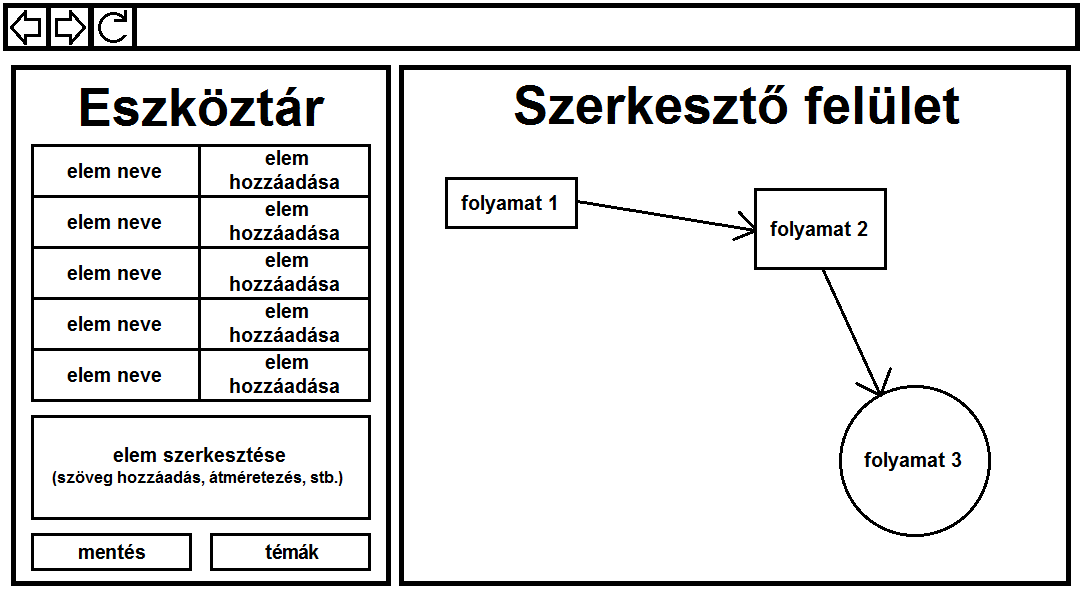
\includegraphics[scale=0.5]{images/sematikus.png}
\caption{A gráfszerkesztő sematikus rajza}
\label{fig:sematikus}
\end{figure}

Az ábra alapján máris van egy elképzelésünk a program szerkezetéről. Nézzük is meg annak konkrét felépítését.

Bal oldalon található az \textbf{eszköztár}, amelynek segítségével különböző funkciók érhetőek el. Innen tudjuk irányítani (létrehozni, szerkeszteni) a gráf felépítéséhez szükséges elemeket. Az eszköztárból az alábbi funkciók érhetőek el:

\begin{enumerate}
\item Az eszköztár nagy részét egy táblázat teszi ki, amely két oszloppal, és a felvihető elemek számával megegyező sorral rendelkezik. A két oszlop a következő jelentéssel bír:

\begin{itemize}
\item Az \textbf{elem neve} rész helyére kerül az adott elem (csomópont) megnevezése. Nevük alapján különböztethetőek meg az egyes elemek. Az elemeket egymás alatt célszerű lehet például használati gyakoriság alapján rendezni (a téglalap, mint tevékenység, az egyik leggyakrabban alkalmazott csomópont típus, ez lehetne legfelül).
\item Az \textbf{elem hozzáadása} felirat helyén az adott elem formája jelenik meg. Ez gyakorlatilag egy gomb, melyre rákattintva hozható létre a mellette feltüntetett nevű elem a szerkesztő felületen egy előre meghatározott helyen. Természetesen ez csak egy alapértelmezett hely, ahol megjelenik kattintás után az adott elem, ezt a későbbiekben lehetőségünk van áthelyezni.
\end{itemize}

\item A táblázat alatt található egy kisebb rész az elemek szerkesztésére. Ez akkor jelenik meg, amikor a szerkesztő felületen rákattintunk egy csomópontra, melyet szerkeszteni szeretnénk. Itt az alábi szerkesztési lehetőségek állnak rendelkezésünkre:

\begin{itemize}
\item \textbf{Szöveget} adhatunk hozzá a kijelölt csomóponthoz. Elegendő csak beírni a felvinni kívánt szöveget, és az azonnal megjelenik az adott csomópont közepén. Ez egységes minden csomópontra (tehát mindegyik típushoz tudunk írni szöveget).
\item \textbf{Átméretezhetjük} a kijelölt elemet. Ez csomópontonként eltérő, hogy milyen paramétereket kíván (például téglalap csomópontnál a szélesség és a hosszúság együttes megadása eredményezi az új méretet, kör alakú csomópont esetében viszont elegendő csak egy paramétert, a sugárt megadni).
\end{itemize}

\item Az eszköztár alatt található egy \textbf{mentés} gomb, melynek segítségével elmenthetjük az elkészített gráfot egy adatbázisba az esetleges későbbi módosítások céljából.

\item Végül a mentés gomb mellett egy \textbf{témák} feliratú gomb helyezkedik el, melyre rákattintva választhatjuk ki az elemek különböző témáját, stílusát. Ez egy apróbb felhasználóbarát élményt nyújt azáltal, hogy különböző színű és alakú formák használatát is lehetővé teszi az alapértelmezetteken kívül. Természetesen ez nem folyásolja be a program használatát, csupán a kinézetét változtatja meg a felhasználó általt kívántra.
\end{enumerate}

A \textbf{szerkesztő felület} (vagy más szóval vászon (\textit{canvas})) a létrehozott elemek megjelenítéséért felelős. Kezdetben üres, egyszínű az egész. Ahogy viszont rákattintunk az eszköztárban egy általunk kiválasztott elemre, úgy az megjelenik rajta, és különböző műveleteket tudunk rajta végezni.

\begin{enumerate}
\item Minden létrehozott csomópont egy egyedi azonosítószámot (\textit{ID}-t) kap. Ez alapján lehet őket megkülönböztetni egymástól.

\begin{itemize}
%\item Az ID-t az adott csomópontra való kattintással lehet lekérni. %5. rész
\item Nem kaphat két különböző csomópont ugyanolyan azonosítószámot, annak egyedinek kell lennie.
\item Ha bármilyen attribútuma módosul egy csomópontnak (pozíciója, színe, rajta lévő szövege, stb.), akkor is az ID-jának állandónak kell lennie.
\end{itemize}

\item A csomópontokat tetszés szerint mozgatni lehet a szerkesztő felület teljes területén.

\item A csomópontok között vonalak húzhatóak az egyik végén egy nyíllal.

\begin{itemize}
\item Csak két, általunk kiválasztott csomópontot lehet összekötni vonallal. Megkülönböztetünk \textit{cél}- és \textit{forrás csomópont}ot. Az összekötő vonal végén a nyíl arra az elemre fog mutatni, amelyet később jelölünk ki (tehát a célcsomópontra).
\item Egy csomóponthoz több vonal is tartozhat, amiből a következő pont is következik:
\item Egy csomópont cél- és forrás csomópontként is funkcionálhat.
\item Tehát gyakorlatilag annyi vonal indulhat ki egy csomópontól / érkezhet be egy csomópontba, amennyit csak szeretne a felhasználó.
\end{itemize}

\item Lehetőség van adott csomópont törlésére.

\begin{itemize}
\item Ha már a továbbiakban nincs szükség egy csomópontra, akkor az letörölhető a szerkesztőfelületről.
\item Ilyenkor ha van a csomóponthoz tartozó vonal, akkor az is törlésre kerül (több vonal esetén az összes).
\item A programnak ügyelnie kell arra, hogy egy csomópont törlése után se legyenek a későbbiekben létrehozott csomópontok ID-jai között azonosak.
\end{itemize}

\end{enumerate}

\Section{Miben különbözik az elkészített program a már használatban lévő gráfszerkesztőktől?}

Korábban említettem, hogy a \textit{Draw.io} alkalmazásnak is vannak hiányosságai annak ellenére, hogy rendkívül sok lehetőséget kínál. Most nézzük néhány példát, amik előfordulhatnak akkor, hogyha a felhasználó nem elég körültekintő egy ilyen vagy ehhez hasonló gráfszerkesztő használata közben, és elkövet olyan hibákat a szerkesztés folyamán, amik miatt nem várt eredmény születhet, illetve hogy ezek a hibák miért jelenthetnek problémát.

\begin{enumerate}
\item Nem pontosan köt össze a vonallal két folyamatot.

\begin{itemize}
\item Mivel a Draw.io a vonalakat is a folyamatokhoz hasonló módon kezeli, ezért azt is a felhasználó tetszés szerinti helyre mozgathatja (tehát nem muszáj összekötnie vele két csomópontot, magában is állhat egy vonal). Ezáltal előfordulhat olyan ábra is, aminél a felhasználó a vonal vége és az összekötendő csomópont között figyelmetlenségből egy kis helyet kihagy, így valójában nem kötött össze két folyamatot, ami össze szeretett volna.
\end{itemize}

\item Ha letöröl egy csomópontot, amely össze van kötve egy másikkal, akkor a hozzá tartozó vonal a "levegőben marad", nem fog két meghatározott csomópontot összekötni, ezáltal az alapvető funkciója válik feleslegessé.

\begin{itemize}
\item Az előző ponthoz hasonló probléma merül fel itt is, tehát a vonal nem két csomópont közötti összeköttetést fog megvalósítani.
\end{itemize}

\item Takarásba kerülhet két vagy több csomópont.

\begin{itemize}
\item Előfordulhat ezáltal, hogy nem olvasható el a csomóponton található szöveg teljes egészében, vagy akár az is, hogy egy nagyobb méretű csomópont teljesen eltakar egy kisebb méretűt, ezáltal megfeledkezünk róla. Ha nincs rá szükség, célszerűbb lenne letörölni, ha pedig van, mert például valamilyen információt tartalmaz a rajta található szöveg, akkor a takarás által elveszettnek hihetjük, így megtörténhet az is, hogy még egyszer létrehozzuk, ami felesleges munkát eredményez.
\end{itemize}

\item Nincs legalább egy kezdő- és legalább egy végállapot.

\begin{itemize}
\item Ahhoz, hogy teljes folyamatábrát modellezzünk, szükséges definiálni egy-egy kezdő- és végállapotot.
\end{itemize}

\end{enumerate}

Ezekkel a fent felsorolt, esetlegesen felmerülő hibákkal szemben nézzük meg azt minden egyes pontnál, hogy az elkészített program hogyan igyekszik azokat kiküszöbölni:

\begin{enumerate}
\item Összekötő vonalat csak adott 2 csomópont között lehetséges húzni.

\begin{itemize}
\item Az összekötést a program úgy oldja meg, hogy a felhasználó jelöli ki azt a két csomópontot, amelyet össze szeretne kötni. Ahogy korábban is említettem lesz egy forrás csomópont és egy célcsomópont, e kettő közt fogja kirajzolni a program a vonalat úgy, hogy a célcsomópont felé mutat a vonal végén lévő nyíl.
\end{itemize}

\item Csomópont törlése esetén a hozzákapcsolt vonal is törlésre kerül.

\begin{itemize}
\item Több nyíl esetén az összes törlődik elkerülve ezáltal a vonalak "levegőben maradását".
\end{itemize}

\item A program jelez, hogyha egymásra kerülnek csomópontok.

\begin{itemize}
\item A felhasználót a canvas más színűre változtatásával figyelmezteti a program amiatt, hogy fedésbe került két csomópont.
\end{itemize}

\item Figyelmeztet az alkalmazás ha hiányzik kezdő- vagy végállapot.

\begin{itemize}
\item Az előző ponthoz hasonlóan itt is arról tájékoztatja a felhasználót a program, hogy nem teljes az általa modellezett folyamatábra.
\end{itemize}

\end{enumerate}

A fent említett utóbbi két példa egészen addig fog hibajelzést generálni a felhasználó számára, amíg meg nem szűnteti azokat.

\Section{Egyszerűbb folyamatábra létrehozása lépésről lépésre}

Nézzük meg, hogy az elkészített alkalmazásban a felhasználó hogyan tud létrehozni egy egyszerűbb folyamatbárát. Fontos, hogy ez az alfejezet csak elméletben írja le, hogy hogyan valósítható meg a folyamatmodellezés a program segítségével. Folyamatábrák konkrét létrehozását, használatát, elmentését az 5. fejezet tárgyalja.

A program, ahogy azt a felépítésénél olvashattuk, egy teljesen üres canvas-szal (vászonnal) fogadja a felhasználót kezdetben. Ez maga a szerkesztő felület, ahol a folyamatmodellezés történik, és itt fogjuk látni az elkészített folyamatábránkat végeredményként. Egy egyszerű folyamatábrát az alábbi lépéseket követve tudunk létrehozni (természetesen ezek a lépések csak iránymutatóak, nem kötött sorrendet határoznak meg):

\begin{enumerate}
\item Első lépésben kiválasztjuk azokat az elemeket az eszköztárból, amelyek a modellezéshez szükségesek. Ha teljes folyamatábrát szeretnénk készíteni, akkor célszerű először a kezdő- és a végállapotokat létrehozni (ezek hiányában figyelmeztet minket a program).
\item Ha már tudjuk, hogy nagyjából hány tevékenységet szeretnénk ábrázolni, akkor annak megfelelő számú csomópontot hozzáadhatunk a vászonhoz.

\begin{itemize}
\item Természetesen a későbbiekben módosíthatóak a csomópontok száma újabbak hozzáadásával vagy meglévők törlésével.
\end{itemize}

\item Miután felvittük ezeket az elemeket, elmozgathatjuk azokat egymástól különálló helyekre azért, hogy lássuk mindegyik csomópontot egyszerre az ábrán, és ezáltal be tudjuk határolni, hogy mekkora helyre lesz szükségünk a végső folyamatábránál.

\begin{itemize}
\item Ha nem mozgatjuk el egymásról a csomópontokat, és takarni fogja legalább kettő egymást, akkor az előző alfejezetben a 4. példaként említett figyelmeztetést fogjuk kapni. Ezt elkerülve célszerű minden létrehozott csomópontot azonnal elmozdítani az alapértelmezett helyéről.
\end{itemize}

\item Ezt követően megírhatjuk az egyes csomópontok szövegeit, hogy azok pontosan milyen tevékenységet jelölnek.

\begin{itemize}
\item Igény szerint a csomópontokat át lehet méretezni, de a csomópont automatikusan elkezd szélesedni mielőtt a beleírt karakterek hossza elérné a csomópont széleit.
\end{itemize}

\item Ha ezzel is megvagyunk, célszerű valamilyen szempont alapján (például időrendi sorrend szerint) egymás után elhelyezni a csomópontokat balról jobbra, illetve fentről lefelé.
\item Ezután összekötjük az általunk összekapcsolni kívánt csomópontokat egymással. Ha teljes folyamatábrát szeretnénk kapni, akkor figyeljünk az alábbi szempontokra:

\begin{itemize}
\item Legyen legalább 1-1 kezdő- és végállapot úgy, hogy a kezdőállapotból csak kifelé, a végállapotba pedig csak befelé vezet legalább egy összekötő vonal.
\item Minden csomópontba el lehessen jutni (tehát a kezdő- és a végállapotokat kivéve mindegyik csomópont legalább két másikkal összeköttetésben legyen úgy, hogy legalább egy bevezető és legalább egy kivezető vonal tartozik hozzá).
\item Ne legyen olyan csomópont, amiből már nem lehet végállapotba jutni a vonalakon keresztül.
\end{itemize}
%Ezekért figyelmeztet a program

\item Végül ha minden simítást elvégeztünk a folyamatábránkon (megfelelő méretűekre változtattuk a csomópontokat, az általunk kívánt helyekre mozgattuk őket, stb.) utolsó lépésként már csak el kell azt mentenünk, és készen is vagyunk.
\end{enumerate}

\Section{UX design szempontok a programnál}

Ezen alfejezet megírásához a(z) \cite{uxblog}. forrás blogbejegyzését használtam alapul. Az itt említett szempontok, meghatározások alapján építettem fel ezt a részt, és azt egészítettem ki a dolgozat programjára jellemző tulajdonságokkal, egyéni gondolatokkal.

\SubSection{Mi az a UX design?}

A \textbf{felhasználói élmény tervezés} (\textit{user experience design}, UX design) egy tervezési folyamat, ami a felhasználói elégedettséget hivatott javítani a felhasználó és a termék között azáltal, hogy növeli a használhatóságot, a hozzáférhetőséget és az élményt. Lényegében azt kell megtervezni, hogy az elkészült alkalmazás vagy termék jó benyomást keltsen a felhasználóban bizonyos szempontokat figyelembe véve. Ez azért fontos, mert ha a felhasználó elégedett a termékkel, akkor azt szívesebben, örömmel használja, és a pozitív visszajelzés több szempontból is hasznos tud lenni. A használó számára is élményt nyújt, és a készítő is elégedett lesz a termékével.

Nélkülözhetetlen egy, a UX-szel kapcsolatos fogalmat is megemlíteni: a \textbf{UI}-t. Ez a \textit{user interface} (magyarul: \textbf{felhasználói felület}) rövidítése, amely a program és a felhasználó közötti kommunikációért felelős. Többféle felhasználói felületek létezik (például szöveges, parancssoros, grafikus). Esetünkben \textit{grafikus felhasználói felület}ről beszélhetünk, hiszen a program grafikus (rajzos, szöveges) elemeket tartalmaz, nem kell parancsokat kiadni bizonyos funkciók elérése érdekében.

\SubSection{UX alapkövetelmények}

Nézzük meg, hogy milyen alapkövetelményei vannak a UX-nek egy adott weboldal szemponjából, illetve hogy ezeket az alapkövetelményeknek mennyire felel meg a szakdolgozat programja.

\begin{enumerate}
\item \textbf{Legyen hasznos:} A célközönségnek kell a legnagyobb fókuszban lennie: jelen esetben ez a felhasználók, akik számára készül a program. Ezáltal úgy kell azt megvalósítani, hogy az érdemleges információt tartalmazzon, felkeltse a felhasználó érdeklődését, és így hasznosnak találja a programot.

\begin{itemize}
\item A program hasznosságát az mutatja, hogy az valós szervezeti folyamatok modellezését segíti elő azáltal, hogy lehetővé teszi a folyamatok ábrázolását. Ennek szükségességéről a 2. fejezetben olvashatunk.
\end{itemize}

\item \textbf{Legyen könnyen használható:} Ne legyen túlzsúfolt az oldal, hanem törekedjen az átláthatóságra. Rajta a navigáció legyen következetes és mindenki számára egyértelmű. Ha az alkalmazás nyújtotta lehetőségeket egyszerűen, könnyedén lehet kezelni, az mindenképp pozitív élményt jelent a felhasználó számára.

\begin{itemize}
\item Az alkalmazás nincs túlbonyolítva, kivitelezése átlátható, használata egyszerű. Ami pedig még inkább megkönnyíti a felhasználó eligazodását, hogy a műveletet végrehajtó gombokra ha ráviszi az egérmutatót, akkor azok egy rövid leírást (\textit{tooltip}et) jelenítenek meg számára, amely a könnyebb használatot segíti elő. Például a \textit{mentés} gombnál leírja, hogy mi fog történni annak megnyomása esetén.
\end{itemize}
%tooltip-et megírni a html-ben (title = "asd")
\item \textbf{Legyen kívánatos:} Fontos szempont a testreszabottság. Elvárás lehet a célközönség részéről a kifogástalan esztétikai élmény. Ezáltal lényeges, hogy minél letisztultabb felületet biztosítson az alkalmazás. Nem mindig a legfelkapottabb a célra legmegfelelőbb, viszont kívánatossá teheti a programot.

\begin{itemize}
\item A program ennél az alapkövetelménynél hiányt szenved, ugyanis nem használja a legmodernebb és legnépszerűbb JavaScript könyvtárakat (sőt, egyáltalán nem használ semmilyen könyvtárat). Ugyanakkor megmutatja, hogy az alap JavaScript, HTML Canvas és némi CSS felhasználásával is elkészíthető egy ilyen alkalmazás.
\end{itemize}

\item \textbf{Legyen könnyen kereshető:} Ez az alapkövetelmény azt írja elő, hogy az adott oldalon / alkalmazásban a keresés hatékony legyen. A felhasználók hamar megtalálják azt, amit keresnek, és hogy egyáltalán az adott oldal rendelkezzen a felhasználó számára a keresett információval.

\begin{itemize}
\item Ezt azért teljesíti könnyen a programunk, mert amint betölt az oldal, mindent a szemünk előtt látunk rajta. Alapvetően nincsenek rejtett dolgok, azonnal elkezdhetjük a folyamatmodellezést, minden egyszerűen a kezünk ügyébe kerül. Egyedül a mentés és a csomópont szerkesztés ami bizonyos funkció végrehajtásakor jelenik meg a felhasználó számára, de ezt az 5. fejezet részletesen tárgyalja majd.
\end{itemize}

\item \textbf{Legyen hozzáférhető:} Vagyis mindenki számára elérhető. A blogbejegyzés különös hangsúlyt fektet a fogyatékkal élőkre, hiszen számukra kellene leginkább biztosítani a könnyű kezelhetőséget és használhatóságot. Ennek ellenére mégsem teljesül sok weboldal esetében ez az alapkövetelmény.

\begin{itemize}
\item Az alkalmazásunk, mint ahogy azt a korábbi pontokban is már olvashattuk, egyszerű használatot és könnyű megértést kínál a felhasználó számára. Ezáltal bárki percek alatt megtanulhatja azt kezelni úgy, hogy képes legyen folyamatábrák készítésére.
\end{itemize}

\item \textbf{Legyen megbízható:} Tehát legyen optimális az oldal azáltal, hogy ne csak szép legyen, hanem gyors is. Ne legyenek rajta felesleges hivatkozások, vagy bármi nem oda illő tartalom, hiszen az összezavarhatja a felhasználót, ami azt eredményezheti, hogy nem fogja többször meglátogatni az oldalt. Ezek elkerülése pozitív benyomást kelthet a felhasználóban, hiszen azt találja az oldalon, amit keresett.

\begin{itemize}
\item Nem tartalmaz a program felesleges mondanivalókat, csupán annyi rajta a tartalom, amennyire szükség van, se több, se kevesebb. A gyorsaságát többek között az adja, hogy nem használ semmilyen külső eszközt (például könyvtárat), illetve nem tartalmaz felesleges nagyméretű objektumokat, amik szintén lassíthatják egyes funkciók elérését.
\end{itemize}

\end{enumerate}
\Chapter{Tervezés}

\Section{Bevezetés}

A specifikációk alapján a programban a felhasználónak kell tudnia csomópontokat hozzáadni, szerkeszteni, és azokat összekötni más csomópontokkal. Továbbá az éppen aktuális munkáját a gráf szerkesztőn el kell tudni menteni, és a program újraindításánál visszatölteni azt. Ez utóbbi megvalósításához szükség van valamilyen "tárolóra", vagyis egy szerverre és egy adatbázisra. Ennél a fejezetnél már nem csak a látható programrészen van a hangsúly, hanem legalább ugyanakkora figyelmet kap a szerver oldal is az adatbázissal, hiszen azok is kiemelkedő részei az alkalmazásnak.

\Section{Technológia és architektúra a szerver oldalon}

Ahhoz, hogy a bevezetőben említett specifikációt megvalósító szoftvert meg tudjuk írni, először kijelöljük a megfelelő technológiákat és az architektúrát. A kliens-szerver architektúra megfelelő erre az alkalmazásra. A kliens egy böngészős frontend, ami egy API-n keresztül tud kommunikálni a backend szerverrel, amely perzisztensen tárolja az adatokat egy relációs adatbázisban. A kliens esetünkben a böngészőben futó \textbf{JavaScript} alkalmazás, míg a szerver egy \textbf{Python} nyelven íródott \textbf{Falcon API}-t használ, valamint \textbf{SQLite} adatbázist a tárolásra.
 
Hogy ez működjön a számítógépünkön, először telepíteni kell a \textbf{Python}-t, és a \textbf{pip}-et. A Python-t egyszerűen le lehet tölteni a hivatalos honlapról\cite{pyt}. Windows felhasználóként a Windowshoz készült 64-bites setup segítségével telepítettem fel az alkalmazást. A \ref{fig:pyt1} ábrán látható, hogy a Python telepítésével egyidejűleg lehetőségünk van a pip telepítésére is, ehhez azonban manuális telepítés szükséges.

\begin{figure}[h]
\centering
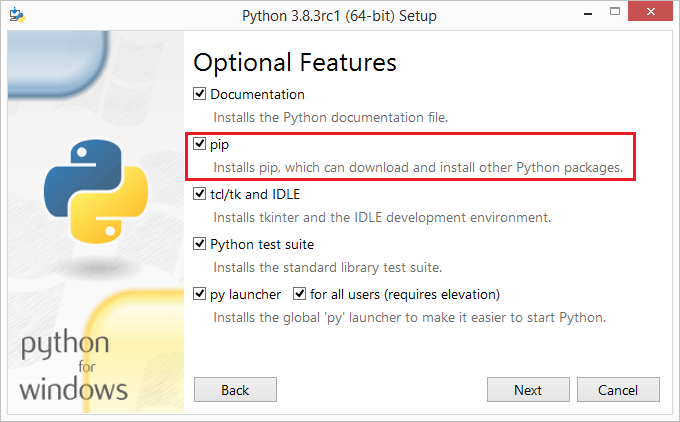
\includegraphics[scale=0.7]{images/python1.png}
\caption{Python telepítése pip-pel együtt}
\label{fig:pyt1}
\end{figure}

A telepítés következő lépésében célszerű bepipálni a 4. pontot, ami a környezeti változókhoz hozzáadja a Python-t (\texttt{Add Python to environment variables}), hiszen ennek elmulasztása esetén láthatósági problémák jelentkezhetnek használat közben.
%Lásd: \ref{fig:pyt2} ábra.

%\begin{figure}[h]
%\centering
%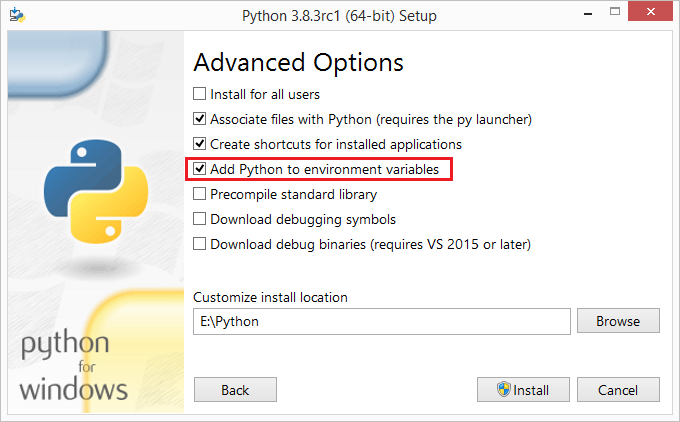
\includegraphics[scale=0.7]{images/python2.png}
%\caption{Python hozzáadása környezeti változókhoz}
%\label{fig:pyt2}
%\end{figure}

Ezek után a program működéséhez elengedhetetlen csomagokat telepítjük: az \textbf{SQLAlchemy}-t és a korábban említett \textbf{Falcon}-t. A telepítés a következő formátum megadásával történik: \texttt{python -m pip install [csomag neve]}

Tehát például a Falcon-t az alábbi parancs kiadása telepíti:

\begin{python}
python -m pip install falcon
\end{python}

Az SQLAlchemy-t pedig így a következő paranccsal fogjuk tudni telepíteni:
\begin{python}
python -m pip install sqlalchemy
\end{python}

Az SQLite3-at is érdemes telepítenünk, ha manuálisan akarjuk létrehozni az adatbázist és a táblákat. A telepítést itt is a hivatalos SQLite oldalon\cite{sqlite} keresztül tehetjük meg.

Ezt követően egy webszerver telepítése következik, például \textbf{waitress} vagy Unix-szerű rendszerek esetében a \textbf{gunicorn}, amivel elérhetjük a programot egy porton keresztül. Esetünkben a 8000-es portot használjuk. A backend szerver egy API-n keresztül szolgálja fel a statikus elemeket is, mint a HTML, CSS, JavaScript fájlokat.
 
Itt láthatjuk az útvonalakat, amelyeken az API felszolgálja a statikus elemeket:

\begin{python}
api.add_route('/js/{filename}', StaticJS())
api.add_route('/css/{filename}', StaticCSS())
api.add_route('/{filename}', StaticHTML())
\end{python}

A backend programban a Falcon keretrendszer kezeli az API-t, és egy adatbázis-kezelő segítségével csatlakozunk az adatbázishoz az alábbi módon:

\begin{python}
api = falcon.API()
dbms = mydatabase.MyDatabase(mydatabase.SQLITE, username='', password='', 
dbname='mydb.sqlite')
\end{python}

Az adatbázis-kezelő osztály tartalmaz metódusokat, amikkel az alapvető műveleteket elvégezhetjük, mint például a lekérdezést, beszúrást, törlést.

\begin{python}
# beszuras, torles
    def execute_query(self, query=''):
            if query == '' : return
            print (query)
            with self.db_engine.connect() as connection:
                try:
                    connection.execute(query)
                except Exception as e:
                    print(e)
def get_all_data(self, table='', query=''):
            query = query if query != '' else "SELECT * 
FROM '{}';".format(table)
            print(query)
            returnData = []
            with self.db_engine.connect() as connection:
                try:
                    result = connection.execute(query)
                except Exception as e:
                    print(e)
                else:   
                    for row in result:
                        print(row) # print(row[0], row[1], row[2])
                        d = dict(row.items())
                        returnData.append(d)
                    result.close()
            print("\n")       
            return returnData
\end{python}

A szerver egy REST API-n keresztül hallgat a kérésekre. Ezen az API-n szolgálja fel a statikus fájlokat, köztük a kliens programot is, és itt kommunikál a klienssel. Az \texttt{/api/nodes} végponton HTTP GET kéréssel felszolgáljuk az adatokat JSON formátumban az alábbi módon:
%Lásd: \ref{fig:get} ábra.

\begin{json}
[
   {
      "text":"folyamatElso",
      "height":50,
      "width":688,
      "radius":0,
      "y":540,
      "x":887,
      "type":"rectangle",
      "id":1
   },
   {
      "text":"folyamatMasodik",
      "height":50,
      "width":156,
      "radius":0,
      "y":512,
      "x":446,
      "type":"rectangle",
      "id":2
   },
   {
      "text":"",
      "height":0,
      "width":0,
      "radius":40,
      "y":122,
      "x":55,
      "type":"start",
      "id":3
   },
   {
      "text":"kezdo",
      "height":0,
      "width":0,
      "radius":40,
      "y":675,
      "x":1195,
      "type":"start",
      "id":4
   }
]
\end{json}

%\begin{figure}[h]
%\centering
%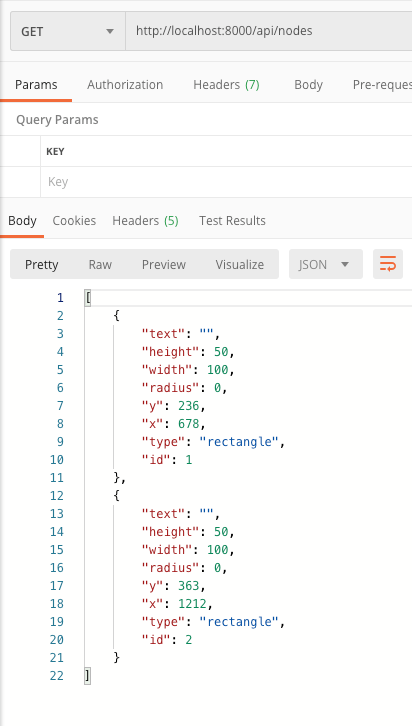
\includegraphics[scale=0.9]{images/get.png}
%\caption{GET kérés}
%\label{fig:get}
%\end{figure}

Ugyanezen a végponton HTTP POST kérés után mentjük az adatokat, amelynek a sikerességéről egy JSON válasz tájékoztat a következőképpen:
%Ez a \ref{fig:post} ábrán látható.

\begin{json}
[
   {
      "text":"",
      "height":50,
      "width":100,
      "radius":0,
      "y":236,
      "x":678,
      "type":"rectangle",
      "id":1
   },
   {
      "text":"",
      "height":50,
      "width":100,
      "radius":0,
      "y":363,
      "x":1212,
      "type":"rectangle",
      "id":2
   }
]
\end{json}

%\begin{figure}[h]
%\centering
%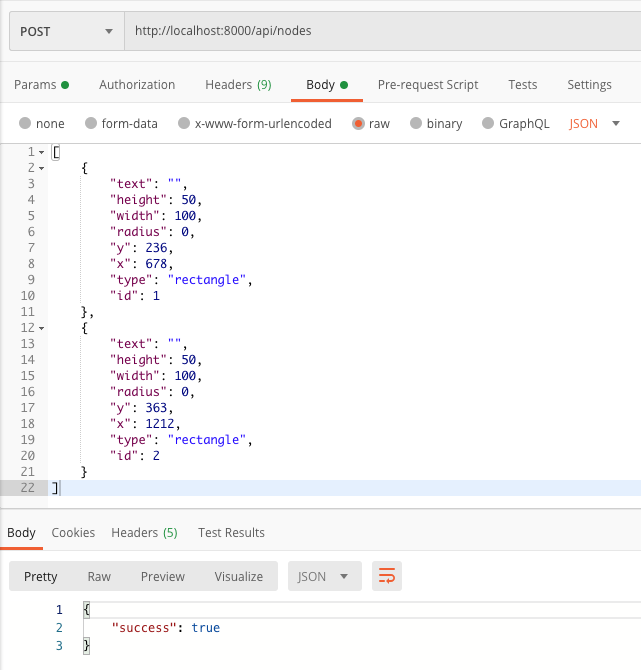
\includegraphics[scale=0.6]{images/post.png}
%\caption{POST kérés}
%\label{fig:post}
%\end{figure}

Az API azért REST, mert követi a REST architektúrát, azaz a web URL és kérés metódus által pontosan azonosítható, mit akar a kliens. Például ha a metódus GET és az URL \texttt{/api/nodes} az azt jelenti, hogy a kliens le szeretné kérni az összes csomópontot.
 
A szerver a már fentebb említett SQLite adatbázissal is kommunikál, itt perzisztensen tároljuk az adatokat, így a következő indításnál is megmarad minden a szerkesztőben.

Az adatbázis két táblát használ, a \textbf{nodes} és az \textbf{edges} táblákat. Először manuálisan kell létrehozni őket, az alábbi ER diagram szerint:

\begin{figure}[h]
\centering
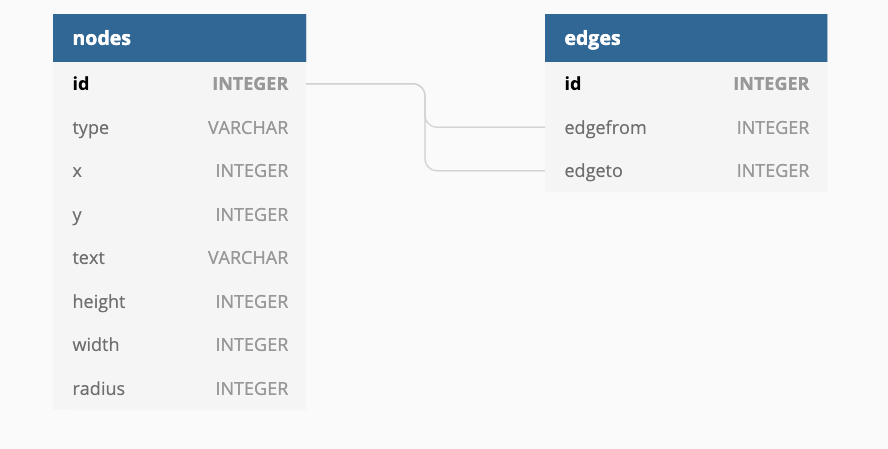
\includegraphics[scale=0.65]{images/sqltables.png}
\caption{SQL táblák ER diagramja}
\label{fig:sql}
\end{figure}

SQLAlchemy-ben így néz ki a fenti séma:

\begin{python}
            nodes = Table(NODES, metadata,
                        Column('id', Integer, primary_key=True),
                        Column('type', String),
                        Column('x', Integer),
                        Column('y', Integer),
                        Column('text', String),
                        Column('height', Integer),
                        Column('width', Integer),
                        Column('radius', Integer)
                        )
            edges = Table(EDGES, metadata,
                        Column('id', Integer, primary_key=True),
                        Column('edgefrom', Integer, 
ForeignKey("nodes.id"), nullable=False ),
                        Column('edgeto', Integer, 
ForeignKey("nodes.id"), nullable=False)
                        ) 
\end{python}

\newpage

\Section{A kliens oldal}
A JavaScript kliens program 9 osztályból áll. Az osztályok mind külön feladatot látnak el. Az \textbf{Editor} osztály körül öleli a többi osztályt, és megosztja közöttük az információkat. A \textbf{Graph} osztály kezeli a szerkesztőt. A szerkesztő és tartalma megrajzolása ebben az osztályban valósul meg. Minden, a szerkesztőn megjelenő elem, ennek az osztálynak valamelyik adattagjában megtalálható. Két fontos adattagja a \textbf{nodes} és \textbf{edges} tömbök, melyek a \textbf{Node} és \textbf{Edge} osztályok, vagy ezen osztályok egyik leszármazottjának a példányait tartalmazzák. A Node osztály tartalmazza a csomópontokat a különböző alakzataival, míg az Edge osztály az alakzatokat összekötő vonalakat valósítja meg.
 
A Node osztálynak 3 közvetlen leszármazottja van: \textbf{Diamond}, \textbf{Rectangle} és \textbf{Circle} (magyarul: rombusz, téglalap és kör) melyek mind implementálják a Node osztály konstruktorát. A Circle osztálynak további két leszármazottja van: a \textbf{Start} és az \textbf{End}, melyek a kezdő- és végállapotokat jelölik.

Ezen osztályoknak mind vannak saját metódusai, melyek ugyanazokat a funkciókat látják el, csak a részletekben térnek el. Ilyen például a \textit{resize()} és \textit{draw()} metódus. Mivel minden alakzatot meg kell rajzolni, vagy adott esetben átméretezni, ezek a metódusok minden alakzatot megvalósító osztályban megtalálhatóak, és a legtöbb funkció végrehajtásakor ezek meg is hívódnak.
 
A frontend egy API-n, \textbf{HTTP kérések}kel kommunikál a szerverrel. A mentés úgy zajlik, hogy a frontend alkalmazás összegyűjti az összes csomópontot és az őket összekötő vonalakat, majd egy objektumot csinál minden egyes csomópontból és vonalból csak a szükséges adatokkal, ezt követően pedig hozzáadja egy tömbhöz. Ezután JSON formátumba alakítja a tömbben lévő objektumokat, amit egy \textbf{HTTP POST} kéréssel elküldünk a szervernek.

A lekéréshez \textbf{HTTP GET} kérést használunk, itt JSON formátumú tömböt kapunk benne a megfelelő adatokat tartalmazó objektumokkal. Ezeket az adatokat visszaalakítjuk, hozzájutva így a megfelelő osztályok konstruktorainak paramétereihez. Ezután a paraméterekkel osztályt hozunk létre belőle, és ezeket az osztályokat hozzáadjuk a Graph osztály nodes és edges adattagjaihoz. Innentől kezdve tudjuk reprezentálni őket a kliens alkalmazással.
\Chapter{JavaScript implementáció}

\Section{A kliens program működése}

A kliens program a következőképpen működik. A \texttt{graphEditor.html} dokumentum betöltése után létrehozzuk az \texttt{Editor} osztály egy példányát. Ezután inicializáljuk a szerkesztőt egy függvény segítségével. Itt beállítjuk a program működéséhez elengedhetetlen adattagokat, események kezelését. Ilyen adattagok a graph, canvas, context, themes.

Végül egy metódus segítségével átméretezzük az adott böngészőablak méretéhez arányosra a canvas-t, biztosítva így, hogy bármilyen méretű képernyőn használható legyen a program.

Az indítás után a program egy aszinkron GET kéréssel lekéri az adatokat a szervertől JSON formátumban. Az adatokból létrehozza a megfelelő osztályokat a konstruktor paraméterekkel. Ezután a csomópontokat hozzáadja a nodes adattaghoz.

\begin{javascript}
function GetEditorData() {
   fetch(apiURL+'/nodes').then(response => response.json())
       .then(data => {
           console.log(data);
           data.map(node => {
               let newNode = {};
               let theme = node["theme"];
               if (theme === "fancy") {
                   editor.graph.selectedtheme = "fancy";
               } else {
                   editor.graph.selectedtheme = "minimal";
               }
               switch (node["type"]) {
                   case "rectangle":
                       newNode = new Rectangle(node["x"],node["y"],node["id"],node["height"], node["width"], node["text"], editor.graph.themes[editor.graph.selectedtheme].rectangleColor);
                       break;
                   case "circle":
                       newNode = new Circle(node["x"],node["y"],node["id"],node["radius"], node["text"], editor.graph.themes[editor.graph.selectedtheme].circleColor);
                       break;
		//...a tobbi csomopontra hasonlokeppen
               }
               let index = editor.graph.nodes.push(newNode) -1;
               editor.graph.selectedIndex = index;
               editor.addTextToNode(node["text"]);
           })
\end{javascript}

Ha ez sikerült, a függvény egy Promise-szal (ígéret) jelzi, és lekérhetjük az összekötő vonalakat. Mivel aszinkron az előző kérés is, előfordulhat olyan, hogy az összekötő vonalak hamarabb megérkeznek, mint maguk a csomópontok, és ez a programban végzetes hibához vezetne. Ezért van szükség a Promise-ra. 

\begin{javascript}
       .then(r => {
\end{javascript}

Ezután egy másik GET kéréssel lekérjük az összekötő vonalakat, és a megfelelő adatokból létrehozzuk az Edge osztály példányait, és hozzáadjuk őket az edges adattaghoz, így a következő rajzolásnál már látszódnak a gráfok. 

A szerkesztő állapotát a következőképpen tudjuk elmenteni: A mentés gombra kattintva először átalakítjuk a nodes és edges adattagokban található osztályokat JSON adattá, majd egy aszinkron POST kéréssel mentjük az adatokat a szerveren.

A csomópontokat megvalósító osztályokat univerzálisan kezeljük: amilyen tulajdonsággal nem rendelkeznek, egyszerűen 0-ra állítjuk, úgyse foglalkozunk velük.

\begin{javascript}
       let nodeJSON = {
           "type": type,
           "x": node.x,
           "y": node.y,
           "id": node.id,
           "text":node.text,
           "height": node.height ? node.height : 0,
           "width": node.width ? node.width : 0,
           "radius": node.radius ? node.radius : 0,
           "theme": node.color.constructor.name === "CanvasGradient" ? "fancy" : "minimal"
       };
       nodes.push(nodeJSON)
\end{javascript}

Az összekötő vonalakat is csak azután küldjük el a szervernek, hogy megbizonyosodtunk arról, hogy a csomópontokat hibamentesen elmentettük. Az SQLite adatbázisban olyan idegen kulcs relációval kapcsolódnak a vonalak a csomópontokhoz, hogy ha a csomópont nem létezik, nem tudjuk elmenteni az összekötő vonalat.
 
Az eseménykezelés a következőképp zajlik: Az egérgomb lenyomásához és felengedéséhez az editor megfelelő metódusát rendeljük.

\begin{javascript}
editor.graph.canvas.addEventListener("mousedown", editor.mouseDown.bind(editor), false);
editor.graph.canvas.addEventListener("mousemove", editor.mouseMove.bind(editor), true);
editor.graph.canvas.addEventListener("mouseup", editor.mouseUp.bind(editor), false);
\end{javascript}
 
Például a \textit{mouseDown} eseménykezelő metódus úgy működik, hogy ha lenyomjuk az egér bal gombját, a függvény újra rajzoltatja a gráfokat, majd kiszámítja, hogy az egér rajta van-e valamely csomóponton. Ha rajta van, az lesz az éppen kijelölt csomópont, és a csomópont osztályban jelez, hogy húzható (\textit{drag}) állapotba került, azaz az éppen kijelölt csomópont követi az egérmutató mozgását.

\begin{javascript}
mouseDown(event)
{
   this.graph.clear();
   this.graph.draw();
   const mouse = this.calcMouseEvent(event);
   this.graph.selectedIndex = null;
   for (let i = 0; i < this.graph.nodes.length; ++i) {
       let node = this.graph.nodes[i];
       if (node.isMouseOnNode(mouse['x'], mouse['y'])){
           this.graph.selectedIndex = i;
       }
   }
   this.graph.dragStart = {
       x: event.clientX - this.graph.canvasPosition.left,
       y: event.clientY - this.graph.canvasPosition.top
   };
   this.graph.drag = true;
}
\end{javascript}

Ha a megfelelő helyre húztuk a csomópontot, és felengedtük az egér bal gombját, a \textit{mouseUp} eseménykezelő metódus jelzi a csomópontokat kezelő osztálynak, hogy a csomópont már nem húzható, azaz nem követi tovább az egeret.

\begin{javascript}
mouseUp(event, context)
{
   this.graph.clear();
   this.graph.draw();
   const mouse = this.calcMouseEvent(event);
   this.graph.drag = false;
   //...
}
\end{javascript}

A csomópontokat úgy tudjuk összekötni, hogy a kiinduló (forrás) csomópontra rákattintunk, miközben nyomva tartjuk a \texttt{Shift} billentyűt. Egy másik (cél)csomópontra kattintva, miközben nyomva tartjuk az \texttt{Alt} billentyűt, kijelölhetjük az összekötendő csomópontot. A \texttt{Ctrl} billentyűvel, és bal egér kattintással törölni tudjuk a csomópontot.

Vonalat törölni szintén a Shift és a Alt billentyűk segítségével lehet (úgy, mint a létrehozásnál), itt viszont a jobb egérgombot kell lenyomnunk a billentyűk mellé.

Ezek között az \texttt{event.which} száma tesz különbséget: Az 1-es a bal egérgombra vonatkozik, a 3-as pedig a jobbra.

\begin{javascript}
if (event.shiftKey === true) {
    this.graph.drawEdge['from'] = this.graph.nodes[selectedIndex];
}
if (event.altKey === true) {
    this.graph.drawEdge["to"] = this.graph.nodes[selectedIndex];
    if (event.which === 1 ){
        this.addEdge(this.graph.drawEdge["from"], this.graph.drawEdge["to"]);
        this.graph.clear();
        this.graph.draw();
    } else if (event.which === 3){
        for (let j = 0; j < this.graph.edges.length; ++j) {
            if(this.graph.nodes[selectedIndex] === this.graph.edges[j].to && this.graph.drawEdge["from"] == this.graph.edges[j].from)
            {
                this.graph.edges.splice(j, 1);
                j = j-1;
                this.graph.clear();
                this.graph.draw();
            }
        }
    }

}
if (event.ctrlKey === true) {
    for (let j = 0; j < this.graph.edges.length; ++j) {
        if(this.graph.nodes[selectedIndex] === this.graph.edges[j].to || this.graph.nodes[selectedIndex] === this.graph.edges[j].from)
        {
            this.graph.edges.splice(j, 1);
            j = j-1;
        }
    }
    this.graph.nodes.splice(selectedIndex, 1);
    this.graph.clear();
    this.graph.draw();
}
\end{javascript}

Az automatikus és manuális méretnövelés a következőképpen működik: Minden csomópontnak van megfelelő metódusa a feladathoz, ami a csomópont saját tulajdonsága alapján elvégzi a feladatot. Például a \textit{widen(length)} metódus elfogad egy paramétert, amely ha túl nagynak bizonyul, növeli a csomópont méretét. A téglalap esetében a szélességet növeljük:

\begin{javascript}
widen(length){
   if(15 > (this.width/length))
   {
       this.width = parseInt(this.width) + 14;
   }
}
\end{javascript}

Viszont például egy körnél a sugarat növeljük:

\begin{javascript}
widen(length){
   if(8 > this.radius / length)
   {
       this.radius += 7;
   }
}
\end{javascript}

Átméretezni egy csomópontot a \textit{resize()} metódussal lehet, itt is hasonlóan a csomópont tulajdonságaihoz megfelelő logikával:

\begin{javascript}
resize(){
   this["width"] = parseInt(document.getElementById("width").value);
   this["height"] =  parseInt(document.getElementById("height").value);
}
\end{javascript}
\Section{Felhasználói kézikönyv a programhoz}

Ez az alfejezet írja le a már korábban többször is említett konkrét kezelését az elkészült gráf szerkesztőnek.

\SubSection{Csomópont hozzáadása}

A bal oldali eszköztárban rákattintunk a hozzáadandó elemre, így az megjelenik a szerkesztő felületen egy előre definiált helyen. Ezt követően az adott csomóponton a bal egérgombot nyomva tartva húzással tudjuk azt mozgatni. Fontos, hogy csak a szerkesztő felület területén belül, annak szélét nem érheti el, tehát nem tudjuk "levágni" a csomópont egy részét a canvas-on túli területre való mozgatással.

\SubSection{Csomópontok összekötése vonallal}

Az összekötésnél figyelembe kell vennünk, hogy a program megkülönböztet forrás- és cél csomópontot, hiszen ez alapján dönti el, hogy a vonal melyik végén lesz a nyíl (vagyis melyik csomópontból melyik másik következik).

\textbf{Forrás csomópont kijelölése:} A szerkesztő felületen a \texttt{Shift} gomb lenyomása mellett az adott csomópontra bal egérgombbal való kattintás fogja kijelölni a forrás csomópontot.

\textbf{Célcsomópont kijelölése:} A Shift gombot elengedve, helyette az \texttt{Alt} gomb lenyomása mellett egy másik csomópontra való kattintás az egér szintén bal gombjával fogja meghatározni a célcsomópontot, vagyis azt, hogy hová lesz bekötve az adott vonal.

Ezt követően már meg is jeleníti a program a kívánt összeköttetést a két csomópont között.

\SubSection{Csomópontok közötti vonal törlése}

Vonalat letörölni hasonlóképpen lehet, mint ahogy azt létrehoztuk. Itt először a \texttt{Shift} gomb lenyomásával egyidejűleg a jobb egérgombot kell megnyomnunk azon a csomóponton, amelyikből a törölni kívánt vonal kiindul. Ezt követően az \texttt{Alt} gomb nyomva tartása mellett szintén jobb egérgombbal való kattintás azon a csomóponton, amelybe vezet a vonal, fogja letörölni az adott vonalat.

A jobb kattintásra megjelenő, legtöbb böngészőbe beépített szerkesztő menü le van tiltva a canvas teljes területén, hogy vonal törlése esetén (ami jobb egérgomb kattintást igényel) ne zavarja meg a felhasználót.

\SubSection{Csomópont törlése}

A törlést a \texttt{Ctrl} gomb nyomva tartása közben a törölni kívánt csomópontra való kattintás teszi lehetővé. Ilyenkor a csomóponthoz kapcsolt vonalak is törlésre kerülnek a csomóponttal együtt.

\SubSection{Szöveg hozzáadása csomóponthoz}

Amelyik csomópontra szöveget szeretnénk írni, azon egy dupla kattintás meg fogja nyitni az eszköztár aljában a szöveg hozzáadásához szükséges részt. Ez a rész addig nem látható, amíg rá nem kattintunk egy csomópontra.

Az itt beírt szöveg azonnal megjelenik az adott csomóponton, illetve, ha a beírt szöveg hossza meghaladja a csomópont szélességét, akkor az automatikusan szélesedni kezd.

Ha lekattintunk az adott csomópontról, majd később visszakattintunk rá (bármelyikre, amelyiken szöveg található), akkor annak a szövege megjelenik azon a helyen, ahol előzetesen beírtuk a csomópont szövegét.

\SubSection{Csomópont átméretezése}

Az átméretezni kívánt csomópontra való dupla kattintással (a szöveg hozzáadásához hasonlóan) érhető el a csomópont átméretezése. Az új méreteket az eszköztár aljában a kattintásra megjelenő felületen lehet megadni.

Hogy legyen mihez viszonyítani, az adott csomópont aktuális mérete megjelenik azon a helyen, ahová majd az új méreteket fogjuk megadni.

A téglalap esetén először annak szélességét, majd a magasságát kell megadnunk. A kör alakú csomópontok (circle, start, end) esetében csak a kör sugarát kell megadnunk.

A csomópontok egy előre definiált minimális méretnél kisebbre nem méretezhetőek. Ezek az értékek az alábbiak:
\begin{itemize}
\item Téglalap esetén 50x50,
\item Rombusz esetén szintén 50x50 (ennek szélessége minden esetben megegyezik a magasságával), 
\item Kör esetén pedig 20
\end{itemize}
Miután beírtuk az új méreteket, az ezek alatt található \texttt{Resize} gomb megnyomása fogja átméretezni a kiválasztott csomópontot.

\SubSection{Téma megváltoztatása}

Az adott témát megváltoztatni az eszköztár alatt található \textbf{graph themes} (gráf témák) felirat melletti legördülő menüben lehetséges. Egy másik téma választása újabb színekkel látja el a csomópontokat. Természetesen egyszerre több témát is használhatunk. Ilyenkor kiválasztunk egyet, felvisszük a kívánt elemeket, majd témát váltunk, és az új téma új színeivel további elemeket adunk hozzá a folyamatábrához.

\SubSection{Folyamatábra mentése}

Az elkészült folyamatábrát a Témák melletti \textbf{Save} gombra kattintva menthetjük el. Ez a funkció minden, a szerkesztő felületen megtalálható elemet (csomópontok, összekötő vonalak, szövegek) elment. Viszont ha a Mentés gomb megnyomása után további szerkesztéseket hajtunk végre, és nem nyomunk ismételten mentés gombot, akkor ez utóbbi módosítások már nem lesznek eltárolva az adatbázisban.

Fontos még megjegyezni, hogy a gráf szerkesztő program a szerver futtatása nélkül is használható, viszont ebben az esetben (értelemszerűen) a mentés funkciót nem tudjuk használni.
\Chapter{Folyamat példák}

\Section{Áttekintés}

Ez a fejezet bemutatja néhány példa segítségével, hogy hogyan és milyen folyamatokat lehet a program elkészülte után annak használatával modellezni. A példák mellé leírás is társul, hogy érthető legyen a modellezett folyamat.

\Section{Első példa}

Először nézzünk egy, már létező példát arra, hogy hogyan is néz ki egy olyan folyamatábra, amely egy üzleti folyamatot modellez. Ehhez tekintsük az alábbi \textit{BPMN} (Business Process Model and Notation) diagramot (\ref{fig:bpmn} ábra).

\begin{figure}[h]
\centering
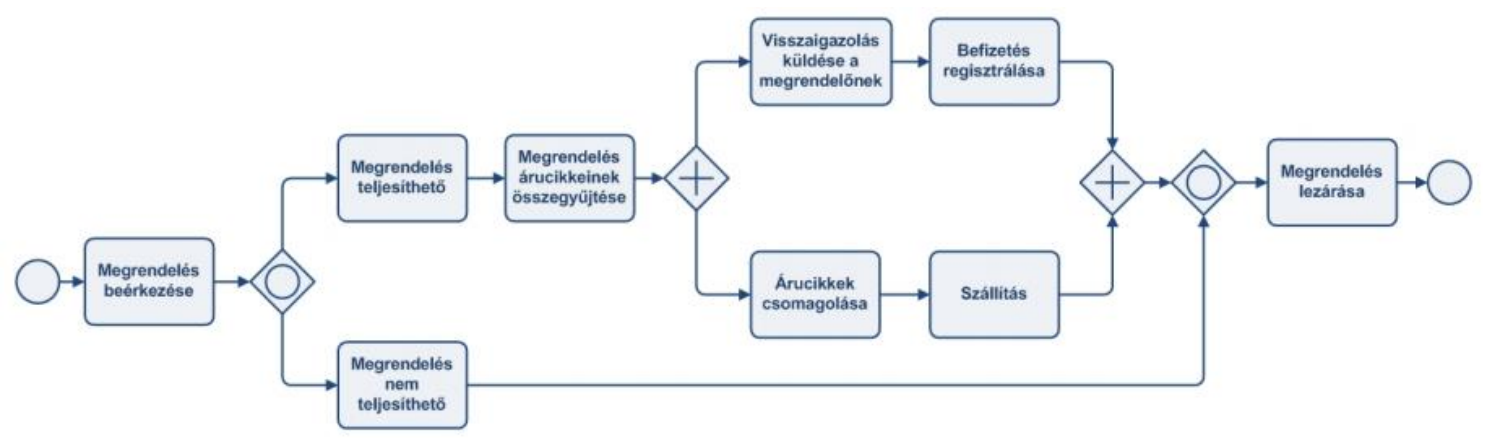
\includegraphics[scale=0.38]{images/BPMN.png}
\caption{BPMN diagram (forrás: \cite{bpmn})}
\label{fig:bpmn}
\end{figure}

Az ábra egy kiváló példa teljes folyamatábrára: Van egy-egy kezdő- és végállapota, minden csomópontba el lehet jutni, és bármelyik csomópontból a végállapotba mehetünk a vonalak és a csomópontok mentén.

A folyamatábrán egy megrendelési folyamatot láthatunk. Első lépésben az adott vállalathoz beérkeznek az általuk megrendelt termékek. Itt máris útelágazáshoz érkezünk: ha a megrendelés nem teljesíthető valamilyen oknál fogva (például aktuálisan nincs rá kapacitása a cégnek, vagy nincs jelen az a személy, aki a megrendeléseket kezeli), akkor máris lezárásra kerül, és végállapotba jutunk a folyamatábrán. Ha viszont minden feltétel adott a megrendeléshez, akkor az teljesíthető. Ekkor összegyűjtik a megrendelés árucikkeit. Ezt követően egy újabb átjáró (vagy elágazás) következik. Láthatjuk, hogy az eddigi két rombusz elem más-más jelölést tartalmaz. Az előbbi egy eldöntendő (igaz vagy hamis) csomópont volt, utóbbi után pedig párhuzamos feladat végrehajtás következik. Egyfelől az összegyűjtött árucikkeket becsomagolják, majd ezt követően elszállítják a megrendelés helyére, ezzel egyidejűleg pedig értesítik a megrendelőt egy visszaigazolással, és regisztrálják a befizetést. Két újabb rombusz alakzat zárja az azonos jellel megjelölt korábbi útválasztó csomópontokat, és végül lezárásra kerül a megrendelés. Az egész folyamat pedig egy kezdő- és egy végállapot közé van fogva.

A fenti ábra után tekintsük meg a \ref{fig:bpmn1} ábrán, hogy pontosan ugyanez a folyamat hogyan modellezhető a szakdolgozat programjának segítségével.

\begin{figure}[h]
\centering
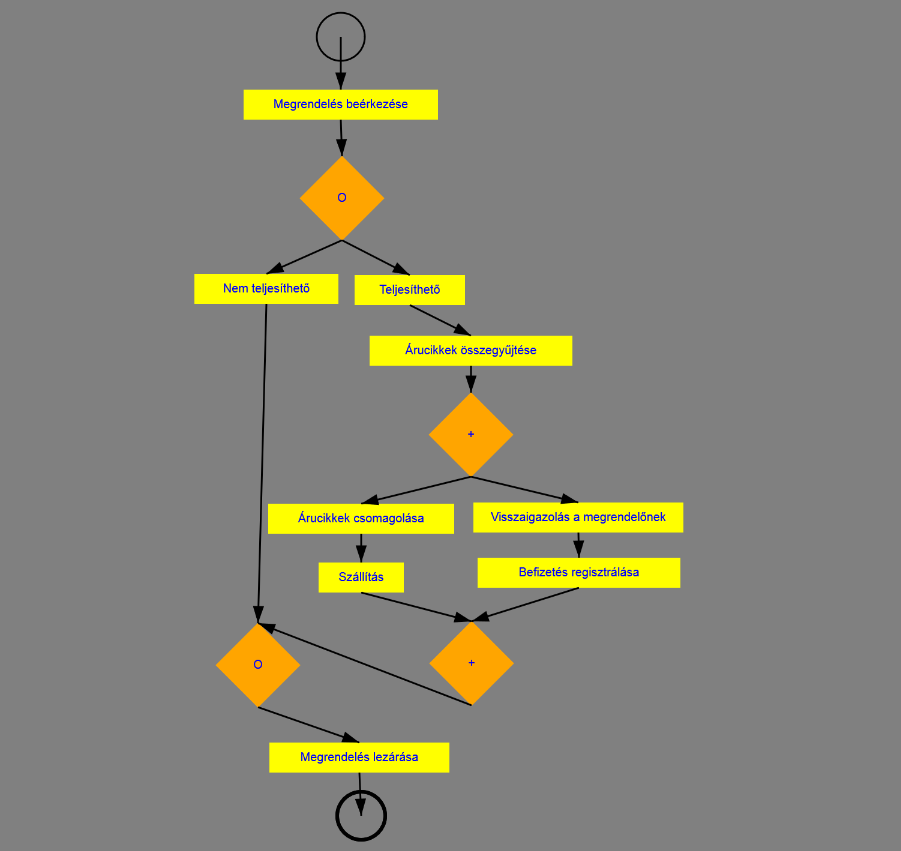
\includegraphics[scale=0.6]{images/pelda1.png}
\caption{BPMN diagram a saját programmal készítve}
\label{fig:bpmn1}
\end{figure}

Némi eltérés felfedezhető a két ábra között. A szakdolgozat alkalmazás színes csomópontokat használ, ami látványosabbá teszi a modellezést, azonban azok összekötésére kisebb hangsúlyt fektet. Előbbi ábrán a csomópontok szövegei több sorba való tagolással vannak megvalósítva, így minden tevékenységet jelölő csomópont azonos méretű. Hosszabb szövegek esetén viszont már nem lesz meg ez az egység. A szakdolgozat programjában ellenben minden csomópont pontosan azonos méretűre hozható a benne lévő szöveg hosszától függetlenül.

\Section{Második példa}

Második példaként hozzunk létre egy létező diagram mintától függetlenül egy folyamatábrát. Tekintsünk egy szerződéskötési folyamatot, melyhez a(z) \cite{xflowutolso} forrásban leírtakat veszem alapul, amely forrás a dolgozat 2. fejezetéhez hasonlóan a(z) \cite{xflower} hivatkozásban található egyik blogbejegyzés.

A folyamat előfeltétele, hogy már egy korábbi (ajánlattevési) folyamatot az ügyfél, akivel a szerződéskötés esedékes, elfogadott. Ezt követően kerül sor a pontos megegyezés (vagyis a szerződés) írásos formában való rögzítésére. Ennek egy egyszerű folyamatát írja le a forrásban említett blogbejegyzés az alábbi lépésekkel:

\begin{enumerate}
\item Első lépésben vázlatot kell készíteni a megegyezett feltételek mellett.
\item Ezt követi a vázlat egyeztetése egy ügyvéddel, vagy egy hozzá értő jogi személlyel.
\item Ha jogilag rendben van minden, akkor a megfogalmazott szöveg kiküldése az ügyfél számára a következő lépés.
\item Az ügyfélnek lehetősége van módosításokat kérvényezni, ebben az esetben a feladat ezek felülvizsgálata, a módosítások egyeztetése, visszaküldése az ügyfélnek.
\item A módosítások után célszerű ismét leellenőrizni, hogy jogilag a helyén van-e a szerződéstervezet.
\item Ha ez is megtörtént, már csak jóvá kell hagynia a két félnek a szerződést, azt aláírásukkal hitelesíteni.
\item Végül iktatásra kerül a szerződés, valamint eltárolásra.
\end{enumerate}
A fenti folyamat ábrázolására többféle lehetőségünk is van. Nézzünk rá egy példát (lásd: \ref{fig:bpmn2} ábra).

\begin{figure}[h]
\centering
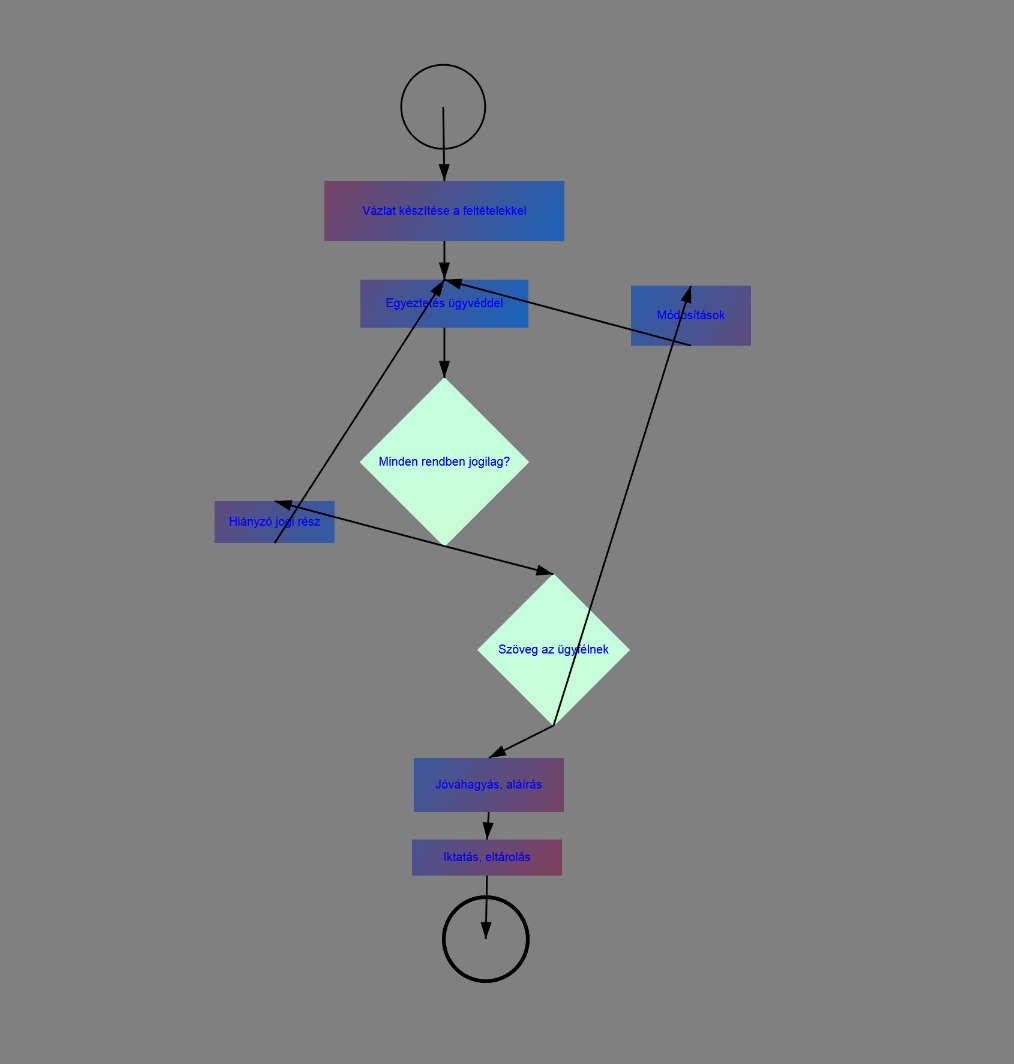
\includegraphics[scale=0.5]{images/pelda2.png}
\caption{Szerződéskötési folyamat modellezése}
\label{fig:bpmn2}
\end{figure}

Először átállítottam a témát, hogy ne csak az alapértelmezett legyen használva, hanem színátmenetes csomópontok is legyenek. Ezután, hogy ne csak tevékenység (téglalap alak) legyen benne, létrehoztam két átjárót is (rombusz alak), ugyanis ha jogi probléma merül fel (például hiányzik a megfogalmazásból valami), akkor ismételten szükség van az ügyvéddel való egyeztetésre, illetve az ügyfélnek küldött szövegen is vagy módosít az ügyfél, vagy következhet a jóváhagyás. Továbbá kihasználtam, hogy a csomópontokat át is lehet méretezni, ezáltal különböző nagyságokat állítottam be az egyes elemeknek.

A fent említett két folyamat példán keresztül még számtalan létezik, és természetesen a felhasználó, aki használni fogja a programot, magától is találhat ki, vagy módosíthat kedvére már létező üzleti folyamat modelleket.
\Chapter{Összefoglalás}

A dolgozat az üzleti folyamatok modellezésének megvalósítását célozta meg elméleti és gyakorlati példák bemutatásával, valamint a hozzá elkészített alkalmazással. Igyekezett felhasználóbarát központúvá tenni az alkalmazást annak működését és kinézetét illetően.

A program kliens oldalon JavaScriptet használt, amihez CSS-t alkalmazott, szerver oldalon pedig egy Python alapú mikrokeretrendszert, a Falcon-t. A gráf szerkesztés során használt adatokat SQLite adatbázisban tárolta.

Az alkalmazás a használat közbeni integritási feltételek ellenőrzésével próbált kiemelkedni a többi hasonló gráf szerkesztő alkalmazás közül. Azonban még sok továbbfejlesztési lehetőség tárul elénk, hiszen ezen ellenőrzések sokaságának köszönhetően további, bonyolultabb validálási feltételeket is meghatározhatunk a jövőben.

Ha lesz legalább egy szoftverfejlesztő csapat, aki felkapja az alkalmazást, és továbbfejleszti az integritási feltételeket ellenőrző részét, akkor már megérte elkészíteni az ehhez alapul szolgáló gráf szerkesztő programot.

\clearpage

\addcontentsline{toc}{chapter}{Irodalomjegyzék}
\bibliographystyle{plain}
\bibliography{dolgozat}
%ez dolgozat.bib volt eddig, de úgy nem működött nekem

\newpage

\pagestyle{empty}

\noindent \textbf{\Large A melléklet tartalma}

\vskip 1cm

\noindent A dolgozat melléklete a következőket tartalmazza:
\begin{itemize}
\item \texttt{dolgozat.pdf:} A szakdolgozat PDF formátumban.
\item \texttt{dolgozat:} A szakdolgozat \LaTeX{} forráskódját tartalmazó jegyzék.
\item \texttt{program:} Az elkészített programok forráskódja.
\end{itemize}
A dolgozat az elkészített program forráskódjával együtt \texttt{GitHub}-on is megtalálható az alábbi címen:

\vskip 0.5cm

\texttt{https://github.com/utrymate/szakdolgozat}

\end{document}
